\documentclass[a4paper]{article}

\usepackage{adjustbox}
\usepackage{algorithm}
\usepackage{algorithmic}
\usepackage{amsmath}
\usepackage{amssymb}
\usepackage{amsthm}
\usepackage{amsfonts}
\usepackage{afterpage}
\usepackage{blindtext}
\usepackage[font=footnotesize,labelfont=bf]{caption}
\usepackage{hyperref}
\usepackage[english]{babel}
\usepackage{bbm}
\usepackage{bigints}
\usepackage{bm}
\usepackage{cite}
\usepackage{color}
\usepackage{float}
\usepackage[left=2cm,right=2cm,top=2cm,bottom=2cm]{geometry}
\usepackage{graphicx}
\usepackage[utf8]{inputenc}
\usepackage{mathtools}
\usepackage{mdframed}
\usepackage{pgfplots} 
\usepackage{subfigure}
\usepackage{stmaryrd}
\usepackage{textcomp}
\usepackage{tikz}
\usepackage{url}
\renewcommand{\proofname}{Proof}
\theoremstyle{plain}
\newtheorem{monTheoNumrote}{Théorème}[section] % Environnement numéroté en fonction de la section
\newtheorem*{monTheoNonNumerote}{Théorème}  % Environnement non numéroté
\newtheorem{The}{Theorem}[section]
\newtheorem*{The*}{Theorem}
\newtheorem{Prop}{Proposition}[section]
\newtheorem*{Prop*}{Proposition} 
\newtheorem{Cor}{Corollary}[section]
\newtheorem*{Cor*}{Corollary}
\newtheorem{Conj}{Conjecture}[section]
\newtheorem{Lem}{Lemma}[section]
\renewcommand{\qed}{\unskip\nobreak\quad\qedsymbol}%
\numberwithin{equation}{section} % Numérote les équations section.numéro.
\theoremstyle{definition}
\newtheorem{Def}{Definition}[section]
\newtheorem{Rem}{Remark}[section]
\newtheorem*{Rem*}{Remark}
\newtheorem*{Lem*}{Lemma}
\newtheorem{Que}{Question}
\newcommand{\enstq}[2]{\left\{#1\mathrel{}\middle|\mathrel{}#2\right\}}
\newcommand{\Lp}[2]{L^#1(#2)}
\newcommand{\Sob}[3]{W^{#1,#2}(#3)}
\newcommand{\Rd}[0]{\mathbb{R}^d}
\newcommand{\RN}[0]{\mathbb{R}^N}
\newcommand{\Rn}[0]{\mathbb{R}^n}
\newcommand{\norm}[1]{\left\|#1\right\|}
\newcommand{\sinc}[0]{\textup{sinc}}
\newcommand{\functionDef}[5]{\begin{array}{lllll}
#1 & : & #2 & \longrightarrow & #3 \\
 & & #4 & \longmapsto &\displaystyle #5 \\
\end{array}}
\newcommand{\Theautorefname}{Theorem}
\newcommand{\Propautorefname}{Proposition}
\newcommand{\Corautorefname}{Corollary}
\newcommand{\Lemautorefname}{Lemma}
\newcommand{\Defautorefname}{Definition}
\newcommand{\N}{\mathbb{N}}
\newcommand{\Z}{\mathbb{Z}}
\newcommand{\D}{\mathbb{D}}
\newcommand{\R}{\mathbb{R}}
\newcommand{\A}{\mathcal{A}_{a,b}}
\newcommand{\Crad}{C^\infty_{c,rad}(B)}
\newcommand{\Lrad}{L^2_{rad}(B)}
\newcommand{\Lradab}{L^2_{rad}(\mathcal{A}_{a,b})}
\newcommand{\duality}[2]{\left\langle #1,#2\right\rangle}
\newcommand{\Hrad}{H^1_{rad}(B)}
\newcommand{\Hzrad}{H^1_{0,rad}(B)}
\newcommand{\rmin}{\delta_{\min}}
\newcommand{\rmax}{\delta_{\max}}
\newcommand{\corr}{\gamma}
\newcommand{\question}[1]{\begin{Que} \ 
#1
\end{Que}}
\newcommand{\abs}[1]{\left\lvert #1 \right\rvert}
\newcommand{\CL}[2]{\textup{CL}\left(\enstq{#1}{#2}\right)}
\newcommand{\Script}[1]{`\texttt{#1}`}
\newcommand{\espace}{\text{ }\qquad} 
\newcommand{\loc}{\text{loc}}
\newcommand{\SL}{\textup{SL}\hspace{1.5pt}}
\newcommand{\DL}{\textup{DL}\hspace{1.5pt}}
\newcommand{\fp}{\underset{\varepsilon \to 0}{\textup{f.p.}}}
\newcommand{\scalProd}[2]{\left(#1|#2\right)}
\newcommand{\toDo}[1]{{\color{red}#1}}
\newcommand{\bs}[1]{\boldsymbol{#1}}
\newcommand{\varInRange}[4]{(#1_{#2})_{#3 \leq #2 \leq #4}}
\newcommand{\from}{\colon}
\newcommand{\Cinf}{C^{\infty}}
\newcommand{\isdef}{\mathrel{\mathop:}=}
\newcommand{\defis}{=\mathrel{\mathop:}}

\renewcommand{\algorithmicrequire}{\textbf{Inputs:}}
\renewcommand{\algorithmicensure}{\textbf{Outputs:}}

\pgfplotsset{compat=1.13}

\title{Square root preconditioners for the Helmholtz integral equation}
\author{Martin Averseng\footnote{CMAP, Ecole polytechnique, Route de Saclay, 91128 Palaiseau Cedex.}}
\begin{document}
\maketitle

\begin{abstract}
	We apply pseudo-differential operators theory to the first-kind integral equations on open curves, allowing us to analyze two new preconditioners and study the convergence orders of a Galerkin method on weighted $L^2$ spaces.  
\end{abstract}

\section*{Introduction}
	
\section{Analytical setting}
\label{sec:analyticalSetting}

The Chebyshev polynomials of first and second kinds are respectively given by
\[T_n(x) = \cos(n \arccos(x)),\]
and 
\[U_n(x) = \dfrac{\sin((n+1) \arccos(x))}{\sqrt{1 - x^2}}\,\]
for $x \in [-1,1]$ \toDo{Inclure citation}. They satisfy
the ordinary differential equations
\begin{eqnarray}
	(1-x^2)T_n'' -xT_n' +n^2T_n &=& 0\\\label{preCheb1}
	(1-x^2)U_n'' -3xU_n' +n(n+2)U_n &=&0 \label{preCheb2}
\end{eqnarray}
Let $\omega$ the operator $u(x) \mapsto \omega(x)u(x)$ with $\omega(x) = \sqrt{1 - x^2}$ and let $\partial_x$ the derivation operator. Then \eqref{preCheb1} and \eqref{preCheb2} can be rewritten under the form
\begin{eqnarray}
	-(\omega\partial_x)^2 T_n &=& n^2T_n\,, \label{cheb1}\\
	-(\partial_x\omega)^2 U_n &=& (n+1)^2U_n\, .\label{cheb2}
\end{eqnarray}
Notice that by $\partial_x\omega$ we do not mean $\omega'(x)$ but the operator \[f \mapsto (\omega f)'\]

\subsection{Spaces $T^s$ and $U^s$}


\subsubsection{Definitions}

Both $T_n$ and $U_n$ are polynomials of degree $n$, and form orthogonal families respectively of the Hilbert spaces 
$$L^2_{\frac{1}{\omega}} \isdef \enstq{u \in L^1_\textup{loc}(-1,1)} {\int_{-1}^{1} \dfrac{\abs{u(x)}^2}{\sqrt{1 - x^2} }dx< + \infty}$$
and 
$$L^2_{\omega} \isdef \enstq{u \in L^1_\textup{loc}(-1,1)} {\int_{-1}^{1} {\abs{u(x)}^2}{\sqrt{1 - x^2} }dx< + \infty}.$$
We denote by $\inner{\cdot}{\cdot}_\frac{1}{\omega}$ and $\inner{\cdot}{\cdot}_\omega$ the inner products in $L^2_{\frac{1}{\omega}}$ and $L^2_{\omega}$ respectively.
The Chebyshev polynomials satisfy
\begin{equation}
	\inner{T_n}{T_m}_\frac{1}{\omega} = \left\{
	\begin{array}{l}
	0 \mbox{ if } n\ne m\\
	\pi \mbox{ if } m=n=0\\
	\pi/2 \mbox{ otherwise}
	\end{array} 
	\right.
\end{equation}
and
\begin{equation}
	\inner{U_n}{U_m}_{\omega} = \left\{
	\begin{array}{l}
	0 \mbox{ if } n\ne m\\
	\pi/2 \mbox{ otherwise}
	\end{array} 
	\right.
\end{equation}
which provides us with the so-called Fourier-Chebyshev decomposition. Any
$u\in L^2_{\frac{1}{\omega}}$ can be decomposed through the first kind Chebyshev series 
\begin{equation}
	u(x) = \sum_{n=0}^{+\infty} \hat{u}_n T_n(x)
	\label{FCseries}
\end{equation}
where the Fourier-Chebyshev coefficients $\hat{u}_n$ are given by 
\[ \hat{u}_n \isdef \begin{cases}
\dfrac{2}{\pi}\displaystyle\int_{-1}^{1} \dfrac{u(x) T_n(x)}{\sqrt{1-x^2}}dx & \text{ if } n \neq 0\,,\\
\dfrac{1}{\pi}\displaystyle\int_{-1}^{1} \dfrac{u(x)}{\sqrt{1-x^2}}dx & \text{ otherwise,}\\
\end{cases}\]
and satisfy the Parseval equality
\[ \int_{-1}^{1} \frac{\abs{u(x)}^ 2}{\sqrt{1-x^2}} dx =  \pi \abs{\hat{u}_0}^2 + \frac{\pi}{2}\sum_{n=1}^{+\infty}\abs{\hat{u}_n}^2\,.\]
When $u$ is furthermore a smooth function, on can check that the series \eqref{FCseries} converges uniformly to $u$. Similarly, any 
function $v\in L^2_{\omega}$ can be decomposed along the $U_n$ as
\[ v(x) = \sum_{n=0}^{+\infty} \check{v}_n U_n(x)\]
where the coefficients $\check{v}_n$ are given by 
\[ \check{v}_n \isdef 
\dfrac{2}{\pi}\displaystyle\int_{-1}^{1} v(x) U_n(x)\sqrt{1-x^2}dx  \]
with the Parseval identity
\[ \int_{-1}^{1} \abs{v(x)}^2\sqrt{1-x^2} dx =  \frac{\pi}{2} \sum_{n=0}^{+\infty}\abs{\check{v}_n}^2\,.\]
The preceding analysis can be generalized to define Sobolev-like spaces. 
\begin{Def}
	For all $s \geq 0$, we may define 
	\[T^s = \enstq{ u \in L^2_\frac{1}{\omega}}{ \sum_{n=0}^{+\infty}(1+n^2)^s \hat{u}_n^2 < + \infty}.\]
	This is a Hilbert space for the inner product
	\[(u,v)_{T^s} = \pi\hat{u}_0 \overline{\hat{v}}_0 + \frac{\pi}{2}\sum_{n=1}^{+\infty}(1+n^2)^s\hat{u}_n \overline{\hat{v}}_n.\]
	We also define a semi-norm 
	\[\abs{u}_{T^s} \isdef \frac{\pi}{2}\sum_{n = 1}^{+ \infty}n^{2s} \abs{\hat{u}_n}^2.\]
	We denote by $T^{\infty}$ the Fr\'echet space $T^{\infty} \isdef \displaystyle\cap_{s \in \R} T^s$, and by $T^{-\infty}$ the set of continuous linear forms on $T^{\infty}$. For $l \in T^{-\infty}$, we define
	\[ \hat{l}_n \isdef 
	\displaystyle\begin{cases}
	\frac{2}{\pi} l(T_n) & \text{ if } n \neq 0\,,\\
	\frac{1}{\pi} l(T_0) & \text{otherwise}\\
	\end{cases}\]
	so that for $u \in T^{\infty}$, 
	\[l(u) = \pi\hat{u}_0 \hat{l}_0 + \frac{\pi}{2}\sum_{n=1}^{+\infty}\hat{u}_n \hat{l}_n.\]
	We denote by $\duality{l}{u}_\frac{1}{\omega}$ the previous bilinear form and use it to identify the dual of $L^2_\frac{1}{\omega}$ to itself. Note that when $s=0$, 
	\[\duality{u}{v}_\frac{1}{\omega} = \int_{-1}^{1} \frac{u(x) l(x)}{\omega(x)}dx\] With this identification, any element of $T^s$ with $s \geq 0$ can also be seen as an element of $T^{-\infty}$.  
	Furthermore, the space $T^{-s}$ can be defined for all $s \geq 0$ as
	\[T^{-s} = \enstq{ u \in T^{-\infty}}{ \sum_{n=0}^{+\infty}{(1 + n^2)^{-s} \abs{\hat{u}_n}^2} < \infty}.\]
	Using the former identification $T^{-s}$ becomes the dual of $T^s$. 
\end{Def}
\noindent In a similar fashion, we define the following spaces:
\begin{Def}
	For all $s \geq 0$, we set
	\[U^s = \enstq{u \in L^2_\omega}{ \sum_{n=0}^{+\infty} (1 + n^2)^s\abs{\check{u}_n}^2 < \infty}.\]
	We extend as before the definition to negative indices by setting $U^{-s}$ to be the dual of $U^s$ for $s\geq 0$, this time with respect to the duality
	\[\duality{u}{v}_\omega = \frac{\pi}{2} \sum_{n=0}^{+\infty} \check{l}_n \check{v}_n\] 
\end{Def}
Let $H^s$ the Sobolev space of periodic functions on the torus $\mathbb{T}_{2\pi} \isdef \mathbb{R} / 2\pi\mathbb{\Z}$, and $H^s_e$ (resp. $H^s_o$) the space of even (resp. odd) functions in $H^s$. Let $e_n(\theta) \isdef e^{in\theta}$. Using the $L^2$ scalar product, the dual of $H^s$ can be identified to $H^{-s}$. The resulting duality product is denoted by $\duality{\cdot}{\cdot}_{L^2(\mathbb{T}_{2\pi})}$ The spaces $T^s$ and $U^s$ are then characterized as follows:
\begin{Lem}
	There exists a linear map $C$ from $T^s$ to $H^s_e$ satisfying
	\[\frac{1}{2\pi}\duality{Cu}{e_{-n}}_{L^2(\mathbb{T}_{2\pi})} = \hat{u}_{\abs{n}}\,.\]
	For $u \in T^s$ and $v \in T^{-s}$, there holds 
	\[\frac{1}{2\pi}\duality{u}{v}_{\frac{1}{\omega}} = \duality{Cu}{Cv}_{L^2(\mathbb{T}_{2\pi})}\,.\] 
	When $u$ is a smooth function, we have 
	\[Cu(\theta) = u(\cos(\theta))\]
	Similarly, there exists a unique bijective isometry $S$ from $U^s$ to $H^s_o$ satisfying
	\[\frac{1}{2\pi}\duality{Su}{e_{0}}_{L^2(\mathbb{T}_{2\pi})} = 0\,,\]
	and for $n \neq 0$,
	\[\duality{Su}{e_{n}}_{L^2(\mathbb{T}_{2\pi})} =\textup{sign}(n) \hat{u}_{\abs{n}-1}\,,\]
	For $u \in T^s$ and $v \in T^{-s}$, there holds 
	\[\duality{u}{v}_{\frac{1}{\omega}} = \duality{Su}{Sv}_{H^s \times H^{-s}}\,.\]
	When $u$ is a smooth function, we have 
	\[Su(\theta) = \sin\theta u(\cos(\theta))\]
	\toDo{Bien vérifier les constantes, déplacer au \autoref{thmChar}}.
\end{Lem}
\begin{Rem}
	The spaces $T^n$ correspond, up to a variable change, to the spaces $H^n_e$ defined in \cite{bruno2012second,atkinson1991numerical,yan1988integral,yan1990cosine} among other works, that is, the restriction of the usual Sobolev space $H^n$ to even periodic functions, as stated in \autoref{thmChar}. 
\end{Rem}


\subsubsection{Basic properties}

Obviously, for any real $s$, if $u \in T^s$ the sequence of polynomials 
\[S_N(x) = \sum_{n=0}^{N} \hat{u}_n T_n(x)\]
converges to $u$ in $T^s$. The same assertion holds for $u \in U^s$ when $T_n$ is replaced by $U_n$. Therefore
\begin{Lem}
	\label{densite}
	$C^{\infty}([-1,1])$ is dense in $T^s$ and $U^s$ for all $s \in \R$.
\end{Lem}
\noindent The polynomials $T_n$ and $U_n$ are connected by the following formulas:
\begin{equation}
\label{TnAsUn}
\forall n \geq 2, \quad T_n(x) = \frac{1}{2}\left(U_n - U_{n-2}\right),
\end{equation}
\begin{equation}
\label{UnAsTn}
\forall n \in \N, \quad U_{2n} = 2\sum_{j = 0}^n T_{2j} - 1, \quad U_{2n+1} = 2\sum_{j=0}^n T_{2j+1}.
\end{equation}
We deduce the following inclusions:
\begin{Lem}
	\label{inclusionsTsUs}
	For all real $s$, $T^s \subset U^s$ and for all $s > 1/2$, $U^s \subset T^{s-1}$.
\end{Lem}
Before starting the proof, we introduce the Cesàro operator $C$ defined on $l^2(\N^{*})$ by
\[(Cu)_n = \frac{1}{n}\sum_{k=1}^n u_k\,.\]
As is well-known, this is a linear continuous operator on $l^2(\N^*)$. Its adjoint
\[(C^* u)_n = \sum_{k = n}^{+ \infty} \frac{u_k}{k} \,,\]
is therefore also continuous on $l^2(\N^*)$. In other words, for all $u \in l^2(\N)$, 
\[ \sum_{n = 1}^{+ \infty} \left(\sum_{k = n}^{+ \infty} \frac{u_k}{k}\right)^2 \leq C \sum_{k = 1}^{+ \infty} u_k^2\, .\]

\begin{proof}
	The first property is immediate from \eqref{TnAsUn}. 
	When $u \in U^{s}$ for $s > 1/2$, the series $\sum \abs{\check{u}_n}$ is converging, allowing to identify $u$ to a function in $T^{-\infty}$, with, in view of \eqref{UnAsTn}, 
	\[\hat{u}_{0} = 2\sum_{n=0}^{+ \infty} \check{u}_{2n}, \quad  \hat{u}_j = 2\sum_{n=0}^{+\infty} \check{u}_{j + 2n} \textup{ for } j \geq 1.\]
	Since $u \in U^s$, the sequence $\left((1+n^2)^{s/2} \abs{\check{u}}\right)_{n \geq 1}$ is in $l^2(\N^*)$. Thus, using the continuity of the adjoint of the Cesàro operator mentioned previously, the sequence $r_n \isdef \left( \sum_{k=n}^{+ \infty} (1+k^2)^{\frac{s-1}{2}} \abs{\check{u}_k}\right)_{ n \geq 0}$ is in $l^2(\N)$. But
	\begin{eqnarray*}
		\norm{u}_{T^{s-1}}^2 &=& \sum_{n=0}^{+ \infty} (1 + n^2)^{s-1} \abs{\hat{u}_n}^2\\ 
		&\leq& 4\sum_{n=0}^{+\infty}(1+n^2)^{s-1} \left(\sum_{k=n}^{+\infty} \abs{\check{u}_k}\right)^2 \\
		&\leq& 4\sum_{n=0}^{+ \infty}\left(\sum_{k=n}^{+\infty}(1+k^2)^{\frac{s-1}{2}} \abs{\check{u}_k})\right)^2.\\
		&=& 4\norm{r_n}^2_{l^2}.
	\end{eqnarray*}	
\end{proof}
\noindent One immediate consequence is that $T^{\infty} = U^{\infty}$.  Moreover, we have the following result:
\begin{Lem}
	\[T^{\infty} = C^{\infty}([-1,1])\,.\]
	\label{LemTinfCinf}
\end{Lem}
\begin{proof}
	If $u \in C^{\infty}([-1,1])$, then we can obtain by induction using integration by parts and \eqref{cheb1}, that for any $k \in \N$
	\[\hat{u}_n = \frac{(-1)^k}{n^{2k}} \int_{-1}^{1} \dfrac{(\omega\partial_x)^{2k} u(x) T_n(x)}{\omega(x)}dx.\]
	Noting that $(\omega \partial_x)^2 = (1-x^2)\partial_x^2 - x \partial_ x$, the function $(\omega \partial_x)^{2k}u$ is $C^{\infty}$, and since $\norm{T_n}_\infty = 1$, the integral is bounded independently of $n$. Thus, the coefficients $\hat{u}_n$ have a fast decay, proving that $C^{\infty}([-1,1]) \subset T^{\infty}$. 
	
	For the converse inclusion, if $u \in T^{\infty}$, the series
	\[ u(x) = \sum_{n=0} \hat{u}_n T_n(x)\]
	is normally converging since $\norm{T_n}_\infty = 1$, so $u$ is a continuous function. This proves $T^{\infty} \subset C^0([-1,1])$. It suffices to show that $u' \in T^{\infty}$ and apply an induction argument. Applying term by term differentiation, we obtain
	\[u'(x) = \sum_{n=1}^{+\infty} n u_n U_{n-1}(x).\] 
	Therefore, $u'$ is in $U^{\infty} = T^{\infty}$. This proves the result.
\end{proof}
\begin{Lem}
	For $s \leq \frac{1}{2}$, the functions of $U^s$ cannot be identified to functions in $T^{-\infty}$. 	
\end{Lem}
\begin{proof}
	Assume by contradiction that the functions of $U^{\frac{1}{2}}$ can be identified to elements of $T^{-\infty}$. Then, there must exist a map $I$ continuous from $U^{\frac{1}{2}}$ to $T^{-\infty}$ with the property 
	\[\forall u \in U^{\infty}, \quad Iu = u.\]
	Now, let us consider for example the function $u$ defined by $\check{u}_n = \frac{1}{n \ln(n)}$. Note that $u$ is in $U^{1/2}$. Let $u_N = \sum_{n = 0}^{N} \check{u_n}U_n$. Then $(u_N)$ is a sequence of elements of $U^{\infty}$ converging to $u$ in $U^{1/2}$. By continuity of $I$, and since $I u_N = u_N$, the sequence $(\duality{u_N}{T_0}_\frac{1}{\omega})_{N\in \N}$ must converge with limit $\duality{Iu}{T_0}$. This is not the case since 
	\[\duality{u_N}{T_0}_\frac{1}{\omega} = \sum_{n=0}^{N} \check{u}_n\duality{U_n}{T_0}_\frac{1}{\omega} = \sum_{k = 0}^{\lfloor \frac{N}{2} \rfloor} \frac{1}{2k \ln(2k)} \]
	is diverging. The result for $s \leq \frac{1}{2}$ comes from the fact that $U^{\frac{1}{2}} \subset U^{s}$ for $s \leq \frac{1}{2}$. 
\end{proof}
Two natural derivation operators arise in our context, that give another link between $T^s$ and $U^s$. They are given by the identities 
\begin{align}
	\partial_x T_n &= n U_{n-1}\,, \label{der1} \\
	-\omega \partial_x \omega U_n &= (n+1)T_{n+1}\,. \label{der2}
\end{align}
The first one is obtained for example from the trigonometric definition of $T_n$. This combined with $-(\omega \partial_x)^2 T_n = n^2 T_n$ gives the second identity. 
\begin{Def}
	\label{derivations}
	For all real $s$, the operator $\partial_x$ can be extended into a continuous map from $T^{s+1}$ to $U^{s}$ defined as 
	\[\forall v \in U^{\infty}, \quad \duality{\partial_x u}{v}_{\omega} \isdef -\duality{u}{\omega \partial_x \omega v}_{\frac{1}{\omega}} \,.\] 
	In a similar fashion, the  operator $\omega \partial_x \omega$ can be extended into a continuous map from $U^{s+1}$ to $T^{s}$ defined as
	\[\forall v \in T^{\infty}, \quad \duality{\omega \partial_x \omega u}{v}_\frac{1}{\omega} \isdef -\duality{u}{\partial_x v}_\omega.\]
\end{Def}
\begin{proof}
	Using the identities \eqref{der1} and \eqref{der2}, one can check that the formulas indeed extend the usual definition of the two operators for smooth functions. We now show that the map $\partial_x$ extended this way is continuous from $T^{s+1}$ to $U^s$. The definition 
	\[\forall v \in U^{\infty}, \duality{\partial_x u}{v} \isdef -\duality{u}{\omega \partial_x \omega v}\]
	gives a sense to $\partial_x u$ for all $u$ in $T^{-\infty}$, as a duality $T^{-\infty} \times T^{\infty}$ product, because if $v \in U^{\infty} (= C^{\infty})$, then $\omega \partial_x \omega v = (1-x^2)v' - xv$ also lies in $C^{\infty} (= T^\infty)$. It remains to check the announced continuity. Letting $w = \partial_x u$, we have, by definition, for all $n$
	\[\check{w}_n = \duality{w}{U_n}_{\omega} = - \duality{u}{\omega \partial_x \omega U_n}_\frac{1}{\omega} = n \duality{u}{T_{n+1}}_\frac{1}{\omega} = n\hat{u}_{n+1}\]
	Obviously, this implies the announced continuity with
	\[ \norm{w}_{U^s} \leq \norm{u}_{T^{s+1}}\,.\]
	The properties of $\omega \partial_x \omega$ on $T^s$ are established in a similar way. 
\end{proof}
The operator $\partial_x$ is not continuous from $T^s$ to $T^{s-1}$. However, the following result holds:
\begin{Cor}
	\label{corDxT2T0}
	The operator $\partial_x$ is continuous from $T^{s+2}$ to $T^s$ for all $s > -1/2 $ and from $U^{s+2}$ to $U^s$ for all $s > - 3/2$. On the other hand, $\omega \partial_x \omega$ is continuous from $T^{s+1}$ to $T^s$ and from $U^{s+1}$ to $U^s$ for all $s \in \R$. 
\end{Cor}
\begin{proof}
	For the continuity of $\partial_x$ from $T^{s+2}$ to $T^s$, we se the continuity of $\partial_x$ from $T^{s+2}$ to $U^{s+1}$ and then of the identity from $U^{s+1}$ to $T^s$. For the continuity of $\partial_x$ from $U^{s+2}$ to $U^s$, we use the same arguments in reverse order. 
	
	On the other hand, we have, for $n \geq 2$,
	\[\omega \partial_x \omega T_n = \omega\partial_x \omega \frac{U_n - U_{n-2}}{2} = \frac{(n+1)T_{n+1} - (n-1)T_{n-1}}{2}\,.\]
	Therefore $\omega \partial_x \omega$ is continuous from $T^{s+1}$ to $T^s$. Finally, $\omega \partial_x \omega$ is continuous from $U^{s+1}$ to $T^s$ and the inclusion $T^s \subset U^s$ is continuous for all $s$.   
\end{proof}
\begin{Lem}
	\label{LemInjectionsContinues}
	For all $\varepsilon >0$, if $u \in T^{\frac{1}{2} + \varepsilon}$, then $u$ is continuous and there exists a constant $C$ such that for all $x \in [-1,1]$,
	\[ \abs{u(x)} \leq C \norm{u}_{T^{1/2 + \varepsilon}}.\]	
	Similarly, if $u \in U^{3/2 + \varepsilon}$, then $u$ is continuous and 
	\[ \abs{u(x)} \leq C \norm{u}_{U^{3/2 + \varepsilon}}.\]
\end{Lem}
\begin{proof}
	Using triangular inequality,
	\[\abs{u(x)} \leq \sum_{n = 0}^{+ \infty} \abs{\hat{u}_n}\]
	since for all $n$, $\norm{T_n}_{L^\infty} = 1$. Cauchy-Schwarz's inequality then yields
	\[\abs{u(x)} \leq \sqrt{\sum_{n= 0}^{+ \infty} \frac{1}{(1+ n^2)^{\frac{1}{2}+ \varepsilon}}} \norm{u}_{T^{\frac{1}{2} + \varepsilon}}.\]
	For the second statement, we use the inclusion $U^{s} \subset T^{s-1}$ valid for $s > 1/2$, as established in \autoref{inclusionsTsUs}. 
\end{proof}	

\subsubsection{Characterization of $T^n$ and $U^n$.}
In this section, we provide a characterization of the spaces $T^s$ and $U^s$ in terms of $L^2$ norms of the derivatives. In what follows, $H^s_p(0,T)$ denotes the space of functions in $H^s(\mathbb{T}_{T})$, where $\mathbb{T}_T$ is the torus $\R / (T\Z)$, $H^s_e(0,T)$ (resp. $H^s_o(0,T)$) is the set of even (resp. odd) functions if $H^s_p(0,T)$.
\begin{Lem}
	\label{omegadxetdxomga}
	The operator $\omega \partial_x$ has a continuous extension from $T^1$ to $T^0$. Similarly, the operator $\partial_x \omega$ has a continuous extension from $U^1$ to $U^0$. 
\end{Lem}
\begin{proof}
	Obviously, the operator $\omega$ maps $L^2_\omega = U^0$ to $L^2_\frac{1}{\omega} = T^0$. This is in fact a bijective isometry with inverse $\frac{1}{\omega}$.
	Since $\partial_x$ is continuous from $T^1$ to $U^0$, we have the announced continuity of $\omega \partial_x$.
	For the second part, we write 
	\[\partial_x \omega = \frac{1}{\omega} \left(\omega \partial_x \omega\right).\]
	Where $\omega \partial_x \omega$ is continuous from $U^1$ to $T^0$, and the multiplication by $\frac{1}{\omega}$ is continuous from $T^0$ to $U^0$. 
\end{proof}
We can now state the main result of this paragraph. For a function $u$ defined on $[-1,1]$, we denote by $Cu$ the function defined on $\mathbb{T}_{2\pi}$ by
\[ Cu(\theta) = u(\cos(\theta))\]
and by $Su$ the function defined as 
\[Su(\theta) \isdef \sin(\theta) Cu(\theta).\]
\begin{Lem}
	A function $u$ belongs to the space $T^n$ if and only if $u = \tilde{u} \circ \arccos$ for some function $\tilde{u} \in H^n_e(0,2\pi)$. In this case, $Cu = \tilde{u}$ and
	\[ \norm{u}_{T_n}\sim \norm{Cu}_{H^n} \mbox{ and } \abs{u}_{T^n} \sim \abs{Cu}_{H^n}.\]
	Similarly, $u$ belongs to  the space $U^n$ if and only if $u = \frac{1}{\sqrt{1 - x^2}} \tilde{u}  \circ  \arccos$  for some function $\tilde{u} \in H^n_o(0,2\pi)$. In this case, $Su = \tilde{u}$ and
	\[\norm{u}_{U_n} \sim \abs{Su}_{H^n}.\]	
	Moreover, if $ u \in T^n$, then $(\omega \partial_x)^n u$ is in $L^2_\frac{1}{\omega}$ and 
	\[ \abs{u}_{T^n}^2 \sim \int_{-1}^{1} \frac{((\omega \partial_x)^n u)^2}{\omega}.\]
	\noindent Similarly, if $u \in U^n$, then $(\partial_x \omega)^n u \in L^2_\omega$ and 
	\[ \norm{u}_{U_n}^2 = \int_{-1}^{1}\omega ((\partial_x \omega)^n u)^2.\]
	\label{thmChar}
\end{Lem}
\begin{proof}
	The first two equivalences stem from the fact that 
	\[\hat{u}_n = \frac{1}{\pi}\int_{-\pi}^{\pi} Cu(\theta) \cos(n \theta), \quad  \check{u}_n = \frac{1}{\pi} \int_{-\pi}^{\pi} Su(\theta) \sin((n+1)\theta)d\theta,\]
	which can be verified by using the change of variables $x = \cos\theta$ in the definitions of $\hat{u}_n$ and $\check{u}_n$. 
	Now, let us show that if $ u \in T^n$, then $(\omega \partial_x)^n$ is in $L^2_\frac{1}{\omega}$. The operator $(\omega \partial_x)^2$ is continuous from $T^s$ to $T^{s-2}$ for all real $s$ which implies the result if $n$ is even. If $n$ is odd, say $n = 2k + 1$, we write $(\omega \partial_x)((\omega \partial_x)^{2})^k$, and conclude using \autoref{omegadxetdxomga}.
	The same kind of proof also shows that if $u \in U^n$, $(\partial_x \omega )^nu \in L^2_\omega$.
	The rest of the proof can be performed by computing the quantities for functions in $C^{\infty}([-1,1])$, performing integrations by parts and concluding with the density of $T^{\infty}$ in $T^s$ and $U^s$. 
\end{proof}
\subsection{Spaces $T^s(\Gamma)$ and $U^s(\Gamma)$}

Let $\Gamma$ an smooth open curve in $\mathbb{R}^2$ parametrized by a smooth $C^\infty$ diffeomorphism $r : [-1,1] \to \Gamma$. We choose $r$ such that $\abs{r'(x)} = \frac{\abs{\Gamma}}{2}$ for all $x$, where $\abs{\Gamma}$ is the length of $\Gamma$. For $u : [-1,1] \to \R$, let $R$ the operator defined by $Ru(x) = u(r(x))$. The tangential derivative on $\Gamma$ is defined as $\partial_\tau = \frac{2}{\abs{\Gamma}}R\partial_x R^{-1}$. Moreover, let $\omega_\Gamma \isdef \frac{\abs{\Gamma}}{2} R^{-1}  \omega(x) R$. The previous results can be generalized to this context:

\begin{Def}
	We say that a function $u : \Gamma \to \mathbb{C}$ belongs to $T^s(\Gamma)$ if the function $R^{-1}u$ belongs to $T^s$. Similarly, we say that $u \in U^s(\Gamma)$ if $R^{-1}u \in U^s$. 
\end{Def}

\begin{The} For all $s \in \R$, $T^s(\Gamma)$ and $U^s(\Gamma)$ are Hilbert spaces for the scalar products 
\[\duality{u}{v}_{T^s(\Gamma)} = \duality{R^{-1}u}{R^{-1}v}_{T^s}\,,\]
\[\duality{u}{v}_{U^s(\Gamma)} = \frac{\abs{\Gamma}^2}{2}\duality{R^{-1}u}{R^{-1}v}_{U^s}\,.\]
With these definitions, 
\[\duality{u}{v}_{T^0(\Gamma)} = \int_{\Gamma} \frac{u(x) v(x)}{ \omega_\Gamma(x)} dx\]
and
\[\duality{u}{v}_{U^0(\Gamma)} = \int_{\Gamma} \omega_\Gamma(x) u(x) v(x) dx\]
thus $T^0(\Gamma) = L^2_\frac{1}{\omega_\Gamma}$ and $U^0(\Gamma) = L^2_{\omega_\Gamma}$. Therefore, $U^0(\Gamma)$ can be identified to the dual of $T^0(\Gamma)$ with respect to the $L^2$ scalar product.
For $s < t$, the injections $T^s(\Gamma) \subset T^t(\Gamma)$ and $U^s(\Gamma) \subset U^t(\Gamma)$ are compact. For $n \in \N$, an equivalent scalar product on $T^n$ and $U^n$ is 
\[\duality{u}{v}_{T^n} = \int_{\Gamma} \frac{u(x)v(x) + (\omega_\Gamma \partial_\tau)^n u(x) (\omega_\Gamma \partial_\tau)^n v(x)}{\omega_\Gamma(x)}d\sigma(x)\,,\]
\[\duality{u}{v}_{U^n} = \int_{\Gamma}(\partial_\tau\omega_\Gamma )^n u(x) (\partial_\tau\omega_\Gamma \partial)^n v(x)\omega_\Gamma(x)d\sigma(x)\,,\]
For all $s \in \R$, $T^s(\Gamma) \subset U^s(\Gamma)$ and for all $s > \frac{1}{2}$, $U^s(\Gamma) \subset T^{s+1}(\Gamma)$. For $s > \frac{1}{2}$, $T^s(\Gamma) \subset C^0(\Gamma)$ and $U^{s+1} \subset C^0(\Gamma)$. Moreover, $T^\infty(\Gamma) = U^\infty(\Gamma) = C^\infty(\Gamma)$. 

\end{The}

\subsection{Periodic pseudo-differential operators}

On the family of spaces $H^s_p(0,T)$, a class of periodic pseudo-differential operators (PPDO) has been introduced in \cite{thrunen1998symbol}, with symbolic calculus. A PPDO on $H^s_p(0,T)$ of order $p$ is an operator of the form 
\[A : u \in H^s_p(0,T) \mapsto \sum_{n \in \Z} \sigma_A(t,n) \hat{u}_n e^{\frac{2in\pi t}{T} }\,.\]
for a "prolongated symbol" $\sigma_A \in C^{\infty}(\mathbb{T}_T \times \R)$ satisfying 
\begin{equation}
\label{SymbolsCond}
	\forall j,k \in \N, \exists C_{j,k} >0 : \quad \abs{\partial_t^j \partial_\xi^k \sigma_A(t,\xi)} \leq C_{j,k}(1 + \abs{\xi})^{p - k}\,.
\end{equation}
Here, $\hat{u}_n = \frac{1}{T}\int_{0}^{T}u(t) e^{-i\frac{2n\pi t}{T}}dt$ are the usual Fourier coefficients of $u$ and 
$${\partial_t \isdef \frac{T}{2i\pi}\frac{\partial}{\partial t}}, \quad  \partial_\xi \isdef \frac{T}{2i\pi}\frac{\partial}{\partial \xi},$$ 
with for $j \geq 1$, $\partial_t^{j+1} = \partial_t \partial_t^j$, and $\partial_\xi^{j+1} = \partial_\xi \partial_\xi^j$. 
The class of symbols that satisfy \eqref{SymbolsCond} is denoted by $\Sigma^\alpha$, and $\Sigma^{-\infty} \isdef \cup_{\alpha \in \Z} \Sigma^\alpha$. The operator corresponding to a symbol $\sigma$ is denoted by $\textit{Op}(\sigma)$ and the set of PPDO of order $\alpha$ is denoted by $\textit{Op}(\Sigma^\alpha)$. 

The prolongated symbol is not unique but is determined uniquely at the integer values of $\xi$ by 
\begin{equation}
	\label{symbolUniqueDetermine}
	\sigma_A(t,n) =  e^{-\frac{2in\pi t}{T}}A(e^{\frac{2in\pi t}{T}})\,.
\end{equation}
as shown in \cite{thrunen1998symbol}, justifying the terminology of "prolongated symbol". $A \in \textit{Op}(\Sigma^\alpha)$ if and only if those values satisfy 
\[\forall j,k \in \N, \exists C_{j,k} > 0 : \abs{\partial_t^j \Delta_n^k \sigma_A(t,n)} \leq C_{j,k}(1 + \abs{n})^{\alpha - k}\,,\] 
where $\Delta_n \phi(t,n) = \phi(t,n+1) - \phi(t,n)$ and for $k \geq 1$, $\Delta^{k+1}\phi = \Delta (\Delta^k \phi)$. That is, if the symbol defined in \eqref{symbolUniqueDetermine} satisfies this condition, then there exists a prolongated symbol satisfying \eqref{SymbolsCond}. Because of this, we will abusively write $\sigma \in \Sigma^p$ for a function $\sigma(t,n)$ that can be prolongated to a function $\tilde{\sigma}(t,\xi) \in \Sigma^p$. An operator in $\textit{Op}(\Sigma^\alpha)$ maps continuously $H_p^s(0,T)$ to $H_p^{s + \alpha}(0,T)$ for all $s \in \R$. The composition of two operators in $\textit{Op}(\Sigma^\alpha)$ and $\textit{Op}(\Sigma^\beta)$ gives rise to an operator in $\textit{Op}(\Sigma^{\alpha+\beta})$. 
If two symbols $a$ and $b$ in $\Sigma^{- \infty}$ satisfy $a - b  \in \Sigma^{\alpha}$, we write $a = b + \Sigma^\alpha$. 
\begin{Def}
	Let $a \in \Sigma^{- \infty}$. If there exists a sequence of reals $(p_j)_{j \in \N}$ such that $p_j < p_{j+1}$ and a sequence of symbols $a_j \in \Sigma^{p_j}$ such that for all $N$, 
	\[a = \sum_{i = 0}^{N}a_i + \Sigma^{p_j + 1}\,,\]
	we then write 
	\[a = \sum_{i = 0}^{+ \infty} a_j \,.\]
	This is called an asymptotic expansion of the symbol $a$. 
\end{Def}

The composition of two periodic pseudi-differential operators $A$ and $B$ with symbols $\sigma_A$ and $\sigma_B$ has a symbol $\sigma_C$ with the following asymptotic expansion
\begin{equation}
	\label{a_diese_b}
	\sigma_C(t,\xi) = \sum_{j = 0}^{+\infty}\frac{1}{j!} \left(\frac{\partial}{\partial \xi}\right)^j \sigma_A(t,\xi) \partial_t^j \sigma_B(t,\xi)\,.
\end{equation}
We will use the following result, see \cite{thrunen1998symbol}:
\begin{The}
	\label{thrunen}
	Consider an integral operator $K$ of the form 
	\[K : u \mapsto \frac{1}{T}\int_{0}^T a(t,s) \kappa(t-s) u(s) ds.\]
	where $a$ is $T$-periodic and $C^{\infty}$ in both arguments and $\kappa$ is a $T$-periodic distribution. Assume that the Fourier coefficients $\hat{\kappa}(n)$ of $\kappa$ can be prolonged to a function $\hat{\kappa}(\xi)$ on $\R$ such that
	\[\forall k \in \N,  \exists C_k > 0: \quad \abs{\partial^k_\xi \hat{\kappa}(\xi)} \leq C_k (1 + \abs{\xi})^{\alpha - k}\,.\]
	for some $\alpha$. Then $K$ is in $\textit{Op}(\Sigma^\alpha)$ with a symbol satisfying the asymptotic expansion
	\begin{equation}
	\label{FormuleIntegralOperatorSymbol}
		\sigma_K(t, \xi) = \sum_{j = 0}^{+ \infty} \frac{1}{j!} \left(\frac{\partial}{\partial \xi}\right)^j \hat{\kappa}(\xi) \partial_s^ja(t,s)_{|s = t}\,.
	\end{equation}
\end{The}
\noindent In particular, taking $\kappa = 1$, we see that for all functions $a \in C^{\infty}(\mathbb{T}_T^2)$
\[Ku = \frac{1}{T}\int_{0}^{T} a(t,s) u(s) ds\]
is in $Op\left(\Sigma^{-\infty}\right)$.

\subsection{Pseudo-differential operators on $T^s(\Gamma)$}

\begin{Lem}
	\label{TransportPPDO_T}
	Let $A$ a PPDO that stabilizes the set of smooth even functions. Then $A$ coincides on this set with the operator $B$ with symbol given by 
	\[\sigma_B(\theta,n) = \frac{\sigma_A(\theta,n) + \sigma_A(-\theta,-n)}{2}\,.\]
	Moreover, $\sigma_B$ admits the following decomposition:
	\[ \sigma_B(n,\theta) = a_1(n,\cos\theta) + i \sin(\theta)a_2(n,\cos\theta) \]
	with 
	\[a_1(x,n) = \frac{\sigma_B(\arccos(x),n) + \sigma_B(\arccos(x),-n)}{2}\]
	\[a_2(x,n) = \frac{\sigma_B(\arccos(x),n) - \sigma_B(\arccos(x),-n)}{2i\sqrt{1-x^2}}\] 
	and $a_1$ and $a_2$ are $\Cinf$. 
\end{Lem}
\begin{proof}
Since $A$ stabilizes the set of even functions, for all even function $u$ we have 
\[Au(\theta) = \frac{Au(\theta) + Au(-\theta)}{2}\,.\]
Thus
\[Au(\theta) = \frac{1}{2}\sum_{n \in \Z} \sigma_A(n,\theta) \hat{u}_n e^{in\theta} + \frac{1}{2}\sum_{n \in \Z} \sigma_A(n,-\theta)\hat{u}_n e^{-in\theta}\,.\]
Since $u$ is even, $\hat{u}_n = \hat{u}_{-n}$, therefore, $Au(\theta) = Bu(\theta)$ where $B$ is the operator with symbol $\sigma_B(n,\theta) = \frac{\sigma_A(n,\theta) + \sigma_A(-n,-\theta)}{2}$. In particular, it satisfies the following symmetry:
\[\sigma_B(-n,-\theta) = \sigma_B(n,\theta)\,.\] 
We write $\sigma_B(n,\theta) = f_B(n,\theta) + g_B(n,\theta)$ where $f_B(n,\theta) = \frac{\sigma_B(n,\theta) + \sigma_B(-n,\theta)}{2}$ and $g_B(n,\theta) = \frac{\sigma_B(n,\theta) - \sigma_B(-n,\theta)}{2}$. Notice that $f_B$ (resp. $g_B$) is even (resp. odd) in both $\theta$ and $n$.
The functions $a_1$ and $a_2$ defined in the lemma satisfy
\[a_1(n,x) = f_B(n, \arccos,x),\quad a_2(n,x) = \frac{g_B(n,\arccos(x))}{i\sqrt{1-x^2}}\,.\]
By \autoref{thmChar}, they lie in $T^\infty$ since $f_B$ (resp. $g_B$) is a smooth even (resp. odd) function and  $f_B(n,\theta) = a_1(n,\cos\theta)$, while $g_B(n,\theta) = i \sin \theta a_2(n,\cos\theta)$. Thus 
\[\sigma_B(n,\theta) = a_1(n,\cos\theta) + i \sin\theta a_2(n,\cos\theta)\,. \]
\end{proof}
We use those results to transport the notion of periodic pseudo-differential operators by the change of variable $x = \cos\theta$. Let $A$ an operator on $T^{-\infty}$, assume that there exists a couple of smooth functions $a_1$ and $a_2$ in $\Cinf([-1,1]\times \N)$ such that for all $n \in \N$,
\[AT_n = a_1(x,n) T_n - \omega^2 a_2(x,n) U_{n-1}\,.\]
Such a (non-unique) couple of functions is called a pair of symbols of $A$. For $n\in \Z$ and $\theta \in [0,2\pi]$, define the symbol $\tilde{\sigma}(a_1,a_2)$ by
\[\tilde{\sigma}(a_1,a_2)(\theta,n) = a_1(\cos\theta,\abs{n}) + i \sin\theta\,\text{sign}(n) a_2(\cos\theta,\abs{n})\,.\]
We say that $(a_1,a_2) \in S^\alpha_T$ if $\tilde{\sigma}(a_1,a_2) \in \Sigma^\alpha$, and $S^{-\infty}_T \isdef \cup_{p \in \Z} S^p_T$. The operator defined by a pair of symbols $(a_1,a_2)$ is denoted by $\textit{Op}_T(a_1,a_2)$ and the set of pseudo-differential operatos of order $p$ in $T^{-\infty}$ by $\textit{Op}(S^\alpha_T)$. 
Then, we have the following properties of $\textit{Op}(S^\alpha_T)$:
\begin{Lem}
	If $A \in \textit{Op}(S^p)$, then letting $\tilde{A} \isdef \textit{Op}(\tilde{\sigma}_A)$, for $u \in T^s$, we have 
	\[C(Au) = \tilde{A} (Cu)\,,\]
	where we recall that for any function $v$ in $T^s$, $Cv(\theta) = v(\cos(\theta))$. 
	Reciprocally, if $A$ is a linear operator that maps $T^\infty$ to itself such that
	$CA = \tilde{A}C$ where $\tilde{A}$ is a PPDO of order $p$, then $A$ is in $\textit{Op}(S^p)$ and if $\sigma_{\tilde{A}}$ is the symbol of $\tilde{A}$, then $A = \textit{Op}(a_1,a_2)$ with the functions $a_1$ and $a_2$ of \autoref{TransportPPDO_T}.
\end{Lem}
\begin{proof}
	For the direct result, by linearity, it suffices to show the equality for $u = T_n$ for some $n \in \N$. In this case, we have $Cu(\theta) = T_n(\cos(\theta)) = \cos(n\theta)$. 
	\[\tilde{A}\left(Cu\right)(\theta) = \frac{\tilde{A}e^{in\theta}+\tilde{A}e^{-in\theta}}{2}\,\]
	which gives, by definition of $\tilde{A}$ and using the determination of the symbol \eqref{symbolUniqueDetermine}, 
	\[\tilde{A}\left(Cu\right)(\theta) = \tilde{\sigma}_A(\theta,n)e^{in\theta} + \tilde{\sigma}_A(\theta,-n)e^{-in\theta}\,.\]
	By definition of $\tilde{\sigma}_A$, this gives 
	\[\tilde{A}\left(Cu\right)(\theta) = a_1(\cos\theta,n)\cos(n\theta) - \sin\theta a_2(\cos\theta,n)\sin(n\theta).\]
	Using the identities $\cos(n\theta) = T_n(\cos\theta)$ and $\sin(n\theta) = \sin\theta U_{n-1}(\cos\theta)$ we obtain
	\[\tilde{A}\left(Cu\right)(\theta) = a_1(\cos\theta,n)T_n(\cos\theta) - (1-\cos^2 \theta) a_2(\cos\theta,n) U_{n-1}(\cos\theta)\,,\]
	as claimed. 
	For the converse result, assume that $CA = \tilde{A}C$ where $\tilde{A}$ is a PPDO of order $p$. Then $\tilde{A}$ stabilizes the set of smooth real even functions since $CAu(\theta) = Au(\cos\theta)$ is real and even and $A$ maps smooth functions to smooth functions. Let $B$, $a_1$ and $a_2$ be defined as in \autoref{TransportPPDO_T} for the operator $\tilde{A}$. Using the same calculations as before, we find 
	\[A(T_n)(\cos \theta) = a_1(n,\cos\theta) T_n(\cos\theta) -\omega^2 a_2(n,\cos\theta) U_{n-1}(\cos\theta)\,,\]
	that is $A = \textit{Op}(a_1,a_2)$. Since $\sigma_B \in \Sigma^p$, we get $(a_1,a_2) \in S^p$ as claimed. 
\end{proof}
\begin{Def}
	Let $A : T^{-\infty}(\Gamma) \to T^{-\infty}(\Gamma)$. We say that $A$ is a pseudo-differential operator if $R A R^{-1} \in Op(S^{-\infty}_T)$. Moreover, if $R A R^{-1} \in Op(S^{\alpha}_T)$, we say that $A$ is a pseudo-differential operator of order $\alpha$. The set of pseudo-differential operators of order $\alpha$ on $\Gamma$ is denoted by $S^{\alpha}_T(\Gamma)$.  
\end{Def}

\begin{Def}
	Let $A$ and $B$ in $\textit{Op}(S^{-\infty}_T(\Gamma))$. If $A - B \in \textit{Op}(S^\alpha_T(\Gamma))$, we write 
	\[A = B + T_\alpha \,.\]
\end{Def}

\subsection{Pseudo-differential operators on $U^s(\Gamma)$}

We may define similarly a class of pseudo-differential operators on the spaces $U^s(\Gamma)$. One can show the following result:
\begin{Lem}
	\label{TransportPPDO_U}
	Let $A$ a PPDO that stabilizes the set of smooth odd functions. Then $A$ coincides on this set with the operator $B$ with symbol given by 
	\[\sigma_B(n,\theta) = \frac{\sigma_A(n,\theta) + \sigma_A(-n,-\theta)}{2}\,.\]
	Moreover, $\sigma_B$ admits the following decomposition
	\[\sigma_B(n,\theta) = i a_1(\cos\theta,n) + \sin\theta a_2(\cos\theta,n)\]
	with
	\[a_1(x,n) = \frac{\sigma_B(n,\arccos(x)) + \sigma_B(-n,\arccos(x))}{2i}\]
	\[a_2(n,x) = \frac{\sigma_B(n,\arccos(x)) - \sigma_B(-n,\arccos(x))}{2\sqrt{1-x^2}}\] 
	and $a_1$ and $a_2$ are $\Cinf$. 
\end{Lem}
Let $A$ an operator on $U^{-\infty}$, assume that there exists a couple of smooth functions $a_1$ and $a_2$ in $\Cinf([-1,1]\times \N)$ such that for all $n \in \N$,
\[AU_n = a_1(x,n) U_n + a_2(x,n) T_{n+1}\,.\]
Such a (non-unique) couple of functions is called a pair of symbols of $A$. For $n\in \Z$ and $\theta \in [0,2\pi]$, define the symbol $\tilde{\sigma}(a_1,a_2)$ by
\[\tilde{\sigma}(a_1,a_2)(\theta,n) = i a_1(\cos\theta,\abs{n}) + \sin\theta\,\text{sign}(n) a_2(\cos\theta,\abs{n})\,.\]
We say that $(a_1,a_2) \in S^\alpha_U$ if $\tilde{\sigma}(a_1,a_2) \in \Sigma^\alpha$, and $S^{-\infty}_U \isdef \cup_{p \in \Z} S^p_U$. The operator defined by a pair of symbols $(a_1,a_2)$ is denoted by $\textit{Op}_U(a_1,a_2)$ and the set of pseudo-differential operatos of order $p$ in $T^{-\infty}$  by $\textit{Op}(S^\alpha_U)$. 
\begin{Lem}
	If $A \in \textit{Op}(S^\alpha_U)$, then letting $\tilde{A} \isdef \textit{Op}(\tilde{\sigma}_A)$, for $u \in U^s$, we have 
	\[S(Au) = \tilde{A} (Su)\,,\]
	where we recall that for any function $v$ in $U^s$, $Sv(\theta) = \sin\theta v(\cos(\theta))$. 
	Reciprocally, if $A$ is a linear operator that maps $U^\infty$ to itself such that
	$SA = \tilde{A}S$ where $\tilde{A}$ is a PPDO of order $\alpha$, then $A$ is in $\textit{Op}(S^\alpha_U)$ and if $\sigma_{\tilde{A}}$ is the symbol of $\tilde{A}$, then $A = \textit{Op}_U(a_1,a_2)$ with the functions $a_1$ and $a_2$ of \autoref{TransportPPDO_U}.
\end{Lem}

\begin{The}
	Let $A \in \textit{Op}(S^\alpha_T)$. Then $-\partial_x A \omega \partial_x \omega \in \textit{Op}(S^{\alpha-2}_U)$, and there exists $B \in S^{\alpha + 2}_U$ such that $A = -\omega \partial_x \omega B \partial_x$.
	Similarly, let $A \in \textit{Op}(S^\alpha_T)$. Then $-\omega \partial_x \omega A \partial_x  \in \textit{Op}(S^{\alpha-2}_T)$, and there exists $B \in S^{\alpha + 2}_T$ such that $A = -\partial_x B \omega \partial_x \omega + T^\infty$.
\end{The}
We define as in the previous paragraph the class $S^\alpha_U(\Gamma)$ for a curve $\Gamma$ by using a smooth constant speed parametrization. 

%
%\subsubsection{Classes of operators}
%
%We shall now introduce a class of pseudo-differential operators on the open segment. Essentially, they are, up to a change of variables, the periodic pseudo-differential operators on the torus $\mathbb{T}_{1} = \mathbb{R} / \Z$ that preserve the space of 1-periodic even functions, that is, that map $H^n_e(0,1)$ to itself. A particular property of these pseudo-differential operators is that their symbol is not defined uniquely. We show that a symbolic calculus is still available within this restricted class. 
%
%\begin{Def}
%	Let $p\in \R$. If  $A : T^{\infty} \to T^{-\infty}$ can be extended into a continuous operator from $T^{s}$ to $T^{s + p}$ for any $s \in \R$, we shall say that it is of order $p$ in the scale $T^s$. When an operator is of order $p$ for all $p \in \N$, we call it a smoothing operator. 
%	
%	An operator $A : U^{\infty} \to U^{-\infty}$ which maps continuously $U^s$ to $U^{s+p}$ for all real $s$ is said to be of order $p$ in the scale $U^s$. When the family ($U^s$ or $T^s$) is clear from the context, we simply say that $A$ is of order $p$. 
%\end{Def}
%
%\begin{Def}
%	\label{DefEquivModTp}
%	Let $A$ and $B$ two operators of order $s$ in the scale $T^s$. When the operator 
%	$A - B$ is of order $p \in (0,+\infty]$, we shall write 
%	\[A = B + T_{p}.\]
%	When the scale is $U^s$ instead of $T^s$, we write 
%	\[A = B + U_{p}.\]
%\end{Def}
%
%\label{subsec:classesOfOp}
%
%To ease the computations, we define $T_n = T_{\abs{n}}$ for $n \in \Z$. 
%
%
%\begin{Def}
%	An operator $A \in \mathcal{L}(T^{-\infty})$ belongs to the class $S^{-\infty}$ if there exists a "discrete symbol" $\sigma_A : \N \times \Z$ of $A$ such that, for all $n \in \N$,
%	\[AT_n = \sum_{i \in \Z} \sigma_A(n,i) T_{n-i}\,,\]
%	with furthermore the property that there exists an integer $N$ for which 
%	\[ \abs{i} \geq N \implies \forall n \in \N, \quad \sigma_A(n,i) = 0\,.\]
%\end{Def}
%A single operator $A$ admits infinitely many discrete symbols as shown by the following example. Given $n_0$, let $\sigma$ the symbol defined by 
%\[ \sigma(n,i) = \begin{cases}
%0 & \text{ if } n \neq n_0, i \neq 0 \text{ or } i \neq 2n_0\\
%1 & \text{ if } n = n_0 \text{ and } i = 0\\
%-1 & \text{ if } n = n_0 \text{ and } i = 2 n_0\,.
%\end{cases}\]
%Then, $\sigma$ is a non-trivial discrete symbol of the null operator. Nevertheless, the next result ensures that two symbols of the same operator agree for $n$ large enough. 
%\begin{Lem}
%	\label{NonUniqueness}
%	Let $\sigma$ a discrete symbol of the null operator. Then there exists an integer $N$ such that 
%	\[n \geq N \implies \forall i \in \Z, \quad \sigma(n,i) = 0\,.\]
%	\begin{proof}
%		 By definition of $S^{-\infty}$, there exists an integer $N$ such that 
%		\[ \abs{i} \geq N \implies \forall n \in \N, \quad \sigma_A(n,i) = 0\,.\]
%		Let $n \geq N$, we can write 
%		\[0 = \sum_{i = -N+1}^{N-1} \sigma(n,i) T_{n-i} \,.\]
%		Two Chebyshev polynomials of the same order do not arise in the summation since $\forall i \in [-N +1,N-1]$, $n - i \geq 1$. Orthogonal projection against each $T_{n-i}$ thus yields 
%		\[\forall i \in [-N+1,N-1], \quad \sigma(n,i) = 0\,,\]
%		and by definition of $N$,
%		\[\forall i \in \Z, \quad \sigma(n,i) = 0\,.\]
%		This has been shown for all $n \geq N$ so the claim is proved. 
%	\end{proof}
%\end{Lem}
%
%An alternative definition is given as follows 
%\begin{Def}
%	An operator $A$ belongs to $S^{-\infty}$ if there exists two functions $a_1, a_2 : \R \times \N \to \R$ and an integer $N$ such that for all $n$, $a_1(n,\cdot)$ and $a_2(n,\cdot)$ are polynomials of order at most $N$, and such that, for $n \geq 1$, 
%	\[AT_n(x) = a_1(n,x)T_n(x) + a_2(n,x) \omega^2 U_{n-1}(x),\]
%	while 
%	\[A T_0(x) = a_1(0,x) T_0 \,.\]
% 	We say that $(a_1,a_2)$ is a couple of semi-discrete symbols of $A$. 
%\end{Def}
%Let us prove the equivalence betwwen the two definitions.
%\begin{proof}
%	We prove that the first definition implies the second one. The calculations can also be made in the reverse order to prove the converse. Let $A\in S^{-\infty}$ and let $\sigma_A$ a discrete symbol of $A$. For $(n,i) \in \N \times \Z$, let 
%	\[f_A(n,i) = \frac{\sigma_A(n,i) + \sigma_A(n,-i)}{2}\,,\]
%	\[g_A(n,i) = \frac{\sigma_A(n,i) - \sigma_A(n,-i)}{2}\,.\]
%	We then have
%	\[\begin{split}
%	AT_n = f_A(n,0) T_n &+ \sum_{i = 1}^{+\infty} f_A(n,i) \left(T_{n+i} + T_{n-i}\right)\\
%	& + \sum_{i = 1}^{+\infty} g_A(n,i) \left(T_{n-i} - T_{n+i}\right)\,.
%	\end{split}\]
%	We use the trigonometric identities
%	\[T_iT_n = \frac{T_{n+i} + T_{n-i}}{2}\,.\]
%	\[\omega^2U_{i-1}U_{n-1} = \frac{T_{n-i} - T_{n+i}}{2}\,,\]
%	to get
%	\[AT_n = a_1(n,x) T_n + \omega^2 a_2(n,x) U_{n-1}\]
%	with 
%	\[a_1(n,x) = f_A(n,0) + 2\sum_{i = 1}^{+\infty}f_A(n,i) T_i(x)\,,\]
%	\[a_2(n,x) = 2\sum_{i = 1}^{+\infty}g_A(n,i) U_{i-1 }(x)\,.\]
%	There exists $N$ such that for each $n$, $f_A(n,i)$ and $g_A(n,i)$ are null for $ \abs{i} \geq N$. This implies that $a_1(n,\cdot)$ and $a_2(n,\cdot)$ are polynomials of degree at most $N$. 
%\end{proof}
%As before, there are non-trivial couple of semi-discrete symbols for the null operator. For example, let $a_1$ and $a_2$ be defined as follows. Fix $n_0$ and take $a_1(x,n) = a_2(x,n) = 0$ for $n \neq n_0$, while 
%\[a_1(n_0,x) = -\omega^2 U_{n_0-1}(x) \,,\] 
%\[a_2(n_0,x) = T_{n_0}(x)\,. \]
%Nevertheless, two couple of semi-discrete symbols of the same operator agree for $n$ large enough:
%\begin{Lem}
%	\label{NonUniqueness2}
%	Let $(a_1,a_2)$ a couple of semi-discrete symbols for the null operator. Then there exists $N$ such that $n \geq N$ implies $a_1(n,x) = a_2(n,x) = 0$. 
%\end{Lem}
%\begin{proof}
%	By definition, there exists an integer $N$ such that for all $n$, $a_1(n,\cdot)$ is a polynomial of order less than $N$. Fix $n \geq N$. We have 
%	\[0 = a_1(n,x) T_n(x) + a_2(n,x)\omega^2 U_{n-1}(x)\]
%	and let $(z_i)$ the $(n+1)$ distinct roots of $\omega^2 U_{n-1}$. Note that $T_n(z_i)$ is non-zero for all $i$, thus, for 
%	\[\forall 1 \leq i \leq n+1, \quad a_1(n,z_i) = 0 \,.\]
%	Thus, $a_1(n,\cdot)$ has $n+1$ distinct roots while being a polynomial of order less than $n$. Therefore, $a_1(n,\cdot) = 0$. This in turn implies that $a_2(n,\cdot) = 0$. 
%\end{proof}
%As $a_1(n,\cdot)$ and $a_2(n,\cdot)$ are required to be polynomials, it is in fact possible to ensure uniqueness of the couple by Euclidean division. We may for example ask that $a_1(n,x)$ has a degree less than $n$. If there exists an admissible couple, then we can change $a_1$ such that this condition be satisfied by writing 
%\[a_1(n,\cdot) = b_1(n,\cdot) + Q(x)\omega^2 U_{n-1}(x)\]
%where $b_1(n,\cdot)$ has a degree less than $n$. Then, letting $b_2(n,x) = a_2(n,x) + Q(x)$, we have exhibited such a couple. Of course, with this condition, the null operator only has trivial semi-discrete symbols, by the same arguments as in the proof of the previous lemma. In practice, this uniqueness condition does no seem to bear any special interest. 
%
%Notice that the action of $A$ on a function $u$ is given in terms of a couple of semi-discrete symbols $(a_1, a_2)$ by 
%\[Au(x) = \sum_{n = 0}^{+ \infty} a_1(n,x) \hat{u}_n T_n(x) + \omega^2 \sum_{n = 1}^{+ \infty} a_2(n,x) \hat{u}_n U_{n-1}(x)\, .\]
%Letting $x = \cos(\theta)$ we have 
%\[\begin{split}
%Au (\cos(\theta)) =  &\sum_{n = 0}^{+ \infty} a_1(n,\cos(\theta)) \hat{u}_n \cos(n\theta)\\ 
%&+ \sum_{n = 1}^{+ \infty} \sin(\theta) a_2(n,\cos(\theta)) \hat{u}_n \sin(n\theta)\,.
%\end{split}\]
%Let $\tilde{A}$ the operator defined on $H^n_e(0,1)$ by  
%\[\tilde{A} f (t) = A u (\cos(2\pi t))\]
%where $f(\theta) = u(\cos(2\pi t))$. The Fourier coefficients of $f$ defined by 
%\[\hat{f}_n = \int_{0}^{1}e^{-2i \pi t \cdot n} f(t) dt\]
%satisfy $\hat{f}_n = \frac{\hat{u}_n}{2}$ 
%for $n \neq 0$, and $\hat{f}_0 = \hat{u}_0$. Thus
%\[\begin{split}
%\tilde{A}f (t) =  a(0,x) \hat{f}_0 + &2\sum_{n = 1}^{+ \infty} a_1(n,\cos(2\pi t)) \hat{f}_n \cos(2n \pi t)\\ 
%+&2\sum_{n = 1}^{+ \infty} \sin(2 \pi t) a_2(n,\cos(2 \pi t)) \hat{f}_n \sin(2n \pi t)\,.
%\end{split}\,.\]
%This coincides with a discrete pseudo-differential operator, as defined in \cite{thrunen1998symbol}, with a symbol $\sigma_A$ equal, for $n \neq 0$, to
%\[\sigma_A(n,t) = a_1(\abs{n},\cos(2\pi t)) + i \text{sign}(n) \sin(2\pi t)a_2(\abs{n},\cos(2\pi t))\,.\]
%and for $n= 0$ to
%\[\sigma_A(0,t) = a_1(0,\cos(2\pi t))\,.\]
%Contrary to \cite{thrunen1998symbol}, the resulting symbol $\sigma_A$ is restricted to the class of trigonometric polynomials of bounded degree in the second variable as would result here of our hypothesis for $a_1$ and $a_2$. We need this assumption in order to have a form of uniqueness in our symbols, but consequently, this prevents us from directly applying the results of the previous work. We thus need to prove that our class is still an algebra. 
%
%\begin{Def}
%	\label{defClassSk2}
%	For any real $p$, an operator $A$ belongs to the class $S^{p}$ if one of its discrete symbols $\sigma_A$ satisfies:  \begin{equation}
%		\label{Condition2}
%		\forall (\alpha,i) \in \N \times \Z \,,\exists C_{i,k} >0 : \forall k  \in \Z, \quad  \abs{\Delta_k^\alpha \sigma_A(k,i)} \leq C_{\alpha,i} (1 + k)^{-p - \alpha}\,.
%	\end{equation}
%	Here $\Delta_k$ is the difference operator in the variable $k$ (denoted simply by $\Delta$ when there is only one variable), defined by
%	\[\Delta_k a(k,i) = a(k+1,i) - a(k,i),\]
%	and $\Delta^\alpha_k$ is the $\alpha$-th iterate of $\Delta_k$.
%\end{Def}
%By \autoref{NonUniqueness}, if $A \in S^p$, then any symbol of $A$ satisfies the previous condition. 
%We state an equivalent definition using this time a couple of semi-discrete symbols.
%\begin{Lem}
%	The following conditions are equivalent:
%	\begin{itemize}
%		\item[-] $A \in S^p$
%		\item[-] There exists a couple of semi-discrete symbols $(a_1,a_2)$ of $A$ such that, for $i = 1,2$,
%		\begin{equation}
%		\label{Condition2bis}
%		\forall (\alpha,x) \in \N\,,\exists C_{\alpha} >0 : \forall (k,x)  \in \Z\times[-1,1], \quad  \abs{\Delta_k^\alpha a_i(k,x)} \leq C_{\alpha} (1 + k)^{-p - \alpha}\,.
%		\end{equation}
%	\end{itemize}
%If one of those conditions hold, then the condition \eqref{Condition2bis} holds for any couple of semi-discrete symbols of $A$. 
%\end{Lem}
%\begin{proof}
%	Given a discrete symbol $\sigma_A$ of $A$, $A$ admits the couple of semi-discrete symbols $(a_1,a_2)$ given by 
%	\[a_1(n,x) = f_A(n,0) + 2\sum_{i = 1}^{+\infty}f_A(n,i) T_i(x)\,,\]
%	\[a_2(n,x) = 2\sum_{i = 1}^{+\infty}g_A(n,i) U_{i-1 }(x)\,.\]
%	with $f_A$ and $g_A$ defined as
%	\[f_A(n,i) = \frac{\sigma_A(n,i) + \sigma_A(n,-i)}{2}\,,\]
%	\[g_A(n,i) = \frac{\sigma_A(n,i) - \sigma_A(n,-i)}{2}\,.\]
%	We have by linearity
%	\[\Delta_k^\alpha a_1(k,x) = \Delta_k^\alpha \sigma_A(n,0) + \sum_{i = 1}^{+\infty}\left(\Delta_k^\alpha \sigma_A(n,i)+\Delta_k^\alpha \sigma_A(n,-i) \right) T_i(x)\,.\]
%	We now apply condition \eqref{Condition2} to each term in the sum and with triangular inequality, 
%	\[\abs{\Delta^\alpha_na_1(k,x)} \leq C_\alpha (1 + k)^{-p-\alpha}\]
%	with $C_\alpha = \sum_{i = 0}^{+ \infty}C_{\alpha,i}$, where $C_{\alpha,i}$ are the constant from condition \eqref{Condition2} (recall the sum is actually finite). The same kind of computations gives a similar estimate for $a_2$ and the direct implication is proved. Conversely, let $(a_1,a_2)$ a couple of semi-discrete symbols of $A$ satisfying the condition \eqref{Condition2bis}. Then, reversing the computations, $A$ admits the discrete symbol $\sigma_A$ defined for $n \in \N$ and $i \in \Z$ by
%	\begin{equation}
%		\sigma_A(n,i) = f_A(n,\abs{i}) + \text{ sign} (i) g_A(n,\abs{i})
%		\label{combiner}
%	\end{equation}
%	with, for $i \in \N$, (by orthonormal projection),
%	\[f_A(n,i) = \begin{cases}\frac{1}{2 \norm{T_i}^2_\frac{1}{\omega}}\duality{a_1(n,x)}{T_i}_\frac{1}{\omega}& \text{ if } i \neq 0\\
%	\frac{1}{ \norm{T_0}^2_\frac{1}{\omega}}\duality{a_1(n,x)}{T_0}_\frac{1}{\omega} & \text{ if } i = 0\,.
%	\end{cases}\]
%	and 
%	\[g_A(n,i) = \begin{cases}\frac{1}{2 \norm{U_{i-1}}^2_{\omega}}\duality{a_2(n,x)}{U_{i-1}}_{\omega}& \text{ if } i \neq 0\\
%	0 & \text{ if } i = 0\,.
%	\end{cases}\]
%	Fix $i \in \N^*$. We have for all $k$, by linearity,
%	\[\Delta_k^\alpha f_A(k,i) = \frac{1}{2 \norm{T_i}^2_\frac{1}{\omega}}\duality{\Delta^\alpha_k a_1(k,x)}{T_i}_\frac{1}{\omega}\,.\]
%	Using Cauchy-Schwarz inequality and assumption \eqref{Condition2bis} for $a_1$, we get 
%	\[\abs{\Delta_k^\alpha f_A(k,i)} \leq C_{i}C_\alpha(1+k)^{-p - \alpha}\,,\]
%	with $C_i = \frac{1}{\norm{T_i}}_\frac{1}{\omega}$. Similar estimates can be shown in the same way for $i = 0$ and also for $g_A$. We finally combine them with \eqref{combiner} to conclude for the reverse implication. 
%	The last statement is obvious in view of \autoref{NonUniqueness2}. 
%\end{proof}
%An interpolation procedure gives the following result:
%\begin{Lem}
%	The following propositions are equivalent:
%	\begin{itemize}
%		\item[-] $A \in S^p$
%		\item[-] There exists a couple of functions $(\nu_1(\xi,x),\nu_2(\xi,x))$ defined for $(\xi,x) \in \R^+ \times [-1,1]$, and an integer $N$ such that $a_1$ and $a_2$ are $C^{\infty}$ in $\xi$ and $(\nu_{1|\N \times[-1,1]},\nu_{2|\N \times[-1,1]})$ is a couple of symbols for $A$, with furthermore the property
%		\[\forall \alpha, \exists C_\alpha > 0 : \forall (\xi,x) \in \R+ \times [-1,1], \quad \abs{\partial_\xi^\alpha \nu_i(x,\xi)} \leq C_\alpha (1 + \xi)^{-p - \alpha}\,.\]
%	\end{itemize}
%	We call $(\nu_1,\nu_2)$ a couple of continuous symbols of $A$. 
%\end{Lem}
%\begin{proof}
%	\toDo{Utiliser la procédure d'interpolation du papier PDO discrets.}
%\end{proof}
%
%
%\subsubsection{Symbols that are rational functions of $n$.}
%
%\toDo{Il va peut-être falloir enlever cette section à cause de l'équivalence du lemme précédent.}
%
%Given a discrete symbol $\sigma(n,i)$, is not straightforward to check that the condition \eqref{Condition2} holds for this symbol. We now show that this is the case when $\sigma(n,i)$ is a rational function of $n$. We will repeatedly make use the following forms of Peetre's inequality: for any real $a,b$ and $s$, 
%\begin{equation}
%\label{Peetre1}
%	(1 + \abs{a + b})^s \leq \left(1 + \abs{a}\right)^{\abs{s}} \left(1 + \abs{b}\right)^{s}
%\end{equation} 
%and
%\begin{equation}
%\label{Peetre2}
%\left(1 + \abs{a + b}^2\right)^s \leq 2^{\abs{s}}\left(1 + \abs{a}^2\right)^{\abs{s}} \left(1 + \abs{b}^2\right)^{s}\,.
%\end{equation} 
%\begin{Lem}
%	\label{lemDeltaDerivees}
%	Let $f$ a $C^{\alpha}$ function on $[k,k+\alpha]$. Then for all $k$, 
%	\begin{equation}
%	\label{formule1}
%		\Delta^{\alpha} f(k) =  \int_{x_1 =k}^{k+1}\int_{x_2 = x_{1}}^{x_{1}+1} \cdots \int_{x_\alpha = x_{\alpha-1}}^{x_{\alpha-1}+1} f^{(\alpha)}(x_\alpha)dx_1dx_2 \cdots dx_{\alpha}
%	\end{equation}
%\end{Lem}
%\begin{proof}
%	We show by induction that for all $1 \leq \beta \leq \alpha$, 
%	\begin{equation}
%	\label{hypRec1}
%		\Delta^{\alpha} f(x) = \int_{x}^{x+1} \int_{x_{1}}^{x_{1}+1} \int_{x_{\beta-1}}^{x_{\beta-1}+1} \Delta^{\alpha - \beta} f^{(\beta)}(x_\beta)dx_1dx_2 \cdots  dx_\beta.
%	\end{equation}
%	For $\beta = 1$, we write 
%	\[\Delta^{\alpha}f(x) = \Delta^{\alpha-1}f(x+1) - \Delta^{\alpha-1}f(x),\]
%	therefore,
%	\[\Delta^{\alpha}f(x) = \int_{x}^{x+1} \frac{d}{dx_1}\left(\Delta^{\alpha-1}f\right)dx_1.\]
%	This proves the property for $\beta = 1$. 
%	Let $ 1 \leq \beta < \alpha$ and assume that \eqref{hypRec1} holds for this $\beta$. Then we write
%	\[\Delta^{\alpha - \beta} f^{\beta}(x_\beta) = \int_{x_\beta}^{x_\beta+1} \frac{d}{dx_{\beta}}\Delta^{\alpha - \beta} f^{(\beta)}(x_{\beta+1})dx_{\beta+1}.\]
%	Of course, $\Delta$ and $\frac{d}{dx}$ commute, thus 
%	\[\Delta^{\alpha - \beta} f^{\beta}(x_\beta) = \int_{x_\beta}^{x_\beta+1} \Delta^{\alpha - \beta} f^{(\beta+1)}(x_{\beta+1})dx_{\beta+1}.\]
%	Replacing in \eqref{hypRec1}, this proves the heredity of the property. Finally, taking $\beta = \alpha$ in \eqref{hypRec1} gives the announced result. 
%\end{proof}
%\begin{Cor}
%	\label{lemFracRat}
%	If $f$ is a rational function of degree $p$ which poles are contained in $\mathbb{C} \setminus \N$, then there exists a constant $C_\alpha$ such that for all $k \in \N$, \[\abs{\Delta^{\alpha} f(k)} \leq C_\alpha (1+k)^{p - \alpha}\,.\]
%\end{Cor}
%\begin{proof}
%	Fix a rational fraction $F$ of degree $p$, with poles in $\mathbb{C} \setminus \N$. $F$ is of the form 
%	\[F = P + R\]
%	where $P$ is zero if $p < 0$ and a polynomial of degree $p$ otherwise, and $R$ is a finite linear combination of quantities of the form 
%	\[Q_i(X) = \frac{1}{(X - x_i)^{q}}\]
%	with $x_i \in \mathbb{C} \setminus \N$ and $q \geq -p$. The claimed result is an easy consequence of the following two fact:
%	\begin{itemize}
%		\item[-] If the polynomial $P$ is of degree $p \geq 0$, there holds
%		\[\abs{\Delta^{\alpha} P}(k)  \leq C (1+k)^{p - \alpha},\]
%		\item[-] For the terms $Q_i(X) = \frac{1}{(X - x_i)^{q}},$ there holds
%		\begin{equation}
%		\label{termeQi}
%			\abs{\Delta^{\alpha} Q_i}(k)  \leq C (1+k)^{-q - \alpha}\,.
%		\end{equation}
%	\end{itemize}
%	We first treat the polynomial case. If $\alpha > p$, we have $P^{(\alpha)} = 0$, and thus, by \autoref{lemDeltaDerivees}, $\Delta^{\alpha} P(k) = 0$, and the result is obvious. If $\alpha \leq p$, there exists a constant $C$ such that
%	\[\abs{P^{(\alpha)}(x)} \leq C (1 + x)^{p - \alpha}.\]
%	We inject this in \eqref{formule1}. In the domain of integration, $x_\alpha \leq k + \alpha$, thus
%	\[\abs{\Delta^{q} P}(k) \leq C (1 + (k + \alpha))^{p - \alpha} \leq C (1 + \alpha)^{p-\alpha}(1+k)^{p - \alpha}\]
%	by Peetre's inequality \eqref{Peetre1}. This proves the claim for the polynomial term. 
%	
%	\noindent For $Q_i$, we write:
%	\[Q_i^{(\alpha)}(x) = \frac{(-1)^k p(p+1) \cdots (p+\alpha)}{(x - x_i)^{p+\alpha}}.\]
%	For $x \geq \max \left(1,2 \abs{x_i}\right)$, using Peetre's inequaliy \eqref{Peetre1}, we get
%	\[\abs{Q^{(\alpha)}(x)} \leq \frac{p(p+1) \cdots (p+\alpha)}{(1+x)^{p + \alpha}}.\]
%	We then proceed with the same arguments as for $P$ and conclude that \eqref{termeQi} holds with some constant $C_1$ for all $k  \geq k_0$ where $k_0$ is an integer greater than $\max \left(1,2 \abs{x_i}\right)$. Then \eqref{termeQi} holds for all $k$ with 
%	\[C = \max(C_1,\Delta^{\alpha} Q_i(0), \cdots, \Delta^\alpha Q_i(k_0))\,.\]
%\end{proof}
%
%\subsubsection{Algebraic properties of $S^p$}
%\begin{Lem}
%	If $A\in S^p$, then $A$ is of order $p$ in the scale $T^s$. 
%\end{Lem}
%\begin{proof}
%	Since the sum in the condition (i) is finite, by linearity, showing that the operator $A$ is of order $p$ amounts to proving that the operator $A_i$ defined by
%	\[ \forall k \in \Z, \quad  A_i T_k = a(k,i) T_{k-i} \]
%	is of order $p$. We treat the case $i > 0$, the opposite case being analogous. Let $u \in T^s$ for some $s$, there holds 
%	\[ A_i u = \sum_{k = 0}^{+ \infty} a(i+k,i)\hat{u}_{k + i}T_k + \sum_{k = 0}^{i} a(i - k,i) \hat{u}_{i - k}T_k.\]
%	Let $Vu$ and $Ru$ respectively the two terms of the rhs. Obviously, $R$ is a smoothing operator. Now, for all $k \in \N$ let
%	\[\hat{v}_k \isdef a(i + k,i) \hat{u}_{i + k}.\]
%	Applying Peetre's inequality \eqref{Peetre2},
%	\[(1 + k^2)^{n + s}\abs{\hat{v}_k}^2 \leq 2^{\abs{p+s}}\left(1 + i^2\right)^{\abs{p + s}}\left(1 + (i + k)^2\right)^{p + s} \abs{a(k + i,i)}^2 \abs{\hat{u}_{k+i}}^2.\]
%	Condition (ii) with $\alpha = 0$ yields
%	\[\abs{a(k+i,i)}^2 \leq C\left(1 + (k+i)\right)^{-2p} \leq 2^{\abs{p}}C \left(1 + (k+i)^2\right)^{-p}.\]
%	Therefore, $\norm{V u}_{T^{s + p}} \leq C(1 + i)^{\abs{n + s}} \norm{u}_{T^s}$ which shows that $A$ is of order $p$.
%\end{proof}
%\begin{Lem}
%	\label{LemCompo}
%	If $A \in S^{p}$, $B \in S^{q}$, then $AB$ is in $S^{p + q}$, 
%\end{Lem}
%\begin{proof}
%	A symbol of $AB$ is given by
%	\[c(k,i) = \sum_{j = - \infty}^{+ \infty} a(k - j, i - j) b(k,j).\]
%	This formula is obtained writing the expression of $AB T_n$ using a symbol of $A$ and $B$ and using the identity $T_i T_j = T_{i + j} + T_{i -j}$. 
%	Let $N_a$ such that $\abs{i} \geq N_a \implies a(k,i) = 0$ and let $N_b$ defined in a similar way. Then, it is easy to check that $\abs{i} \geq N_a + N_b \implies c(k,i) = 0$. It remains to check the requirement (ii). Since the sum defining $c$ only has a finite number of non-zero terms, we just have to show that for any $j \in \Z$, the function $c_{j}(k,i) \isdef a(k-j,i-j) b(k,j)$ satisfies
%	\[\forall \alpha \in \N, \forall i,k, \in \Z, \quad  \abs{\Delta_k^\alpha c_{j}(k,i)} \leq C_{i,j,\alpha} (1 + k^2)^{p + q - \alpha}.\]
%	The announced result then follows by linearity. 
%	To prove this, one can check by induction that for any $\alpha \in \N$, $\Delta^\alpha c_j(k,i)$ is of the form 
%	\[\Delta^\alpha_k c_j(k,i) = \sum_{l = 1}^L \lambda_l \Delta_k^{\beta_l}a(k_{l,1},i-j) \Delta_k^{\alpha - \beta_l} b(k_{l,2},j)\]
%	for some coefficients $\lambda_l$, where $L$ is a finite number, and where, for all $l$, $\beta_l \leq \alpha$ while $k_{l,1}$ and $k_{l,2}$ respectively lie in the interval $[k-j,k-j + \beta_l]$ and $[k,k+\alpha - \beta_l]$. Let us fix $l \in [1,L]$. We have
%	\[\abs{\Delta_k^{\beta_l} a(k_{l,1},i-j)} \leq C_{i,j,\alpha,l}(1 + k_1)^{p - \beta_l}\]
%	and by Peetre's inequality
%	\[(1+k_1)^{p - \beta_l} \leq C(1+k)^{p - \beta}(1 + \alpha + \abs{j})^{\abs{p - \beta_l}}.\]
%	The same arguments applied to $b$ lead to 
%	\[\abs{\Delta_k^{\beta} a(k_1,i-j)\Delta_k^{\alpha - \beta} b(k_2,j)} \leq C_{i,j,\alpha,l} (1+k)^{p + q}\]
%	which implies our claim. 
%\end{proof}
%\begin{The}
%	If $A \in S^{p}$ and $B \in S^q$, then $AB - BA$ is in $S^{p + q + 1}$. 
%	\label{CommutPDO}
%\end{The}
%\begin{proof}
%	A symbol of $C= AB - BA$ is given by
%	\[\sigma_{C}(k,i) = \sum_{j = -\infty}^{+\infty} a(k-j,i-j)b(k,j) - \sum_{j = - \infty}^{+\infty} b(k-j,i-j) a(k,j).\]
%	In the second sum, we change the index to $j' = i -j$, yielding 
%	\begin{eqnarray*}
%		\sigma_{C}(k,i) &=& \sum_{j = -\infty}^{+\infty} a(k-j,i-j)b(k,j) - \sum_{j = - \infty}^{+\infty} b(k-i +j',j') a(k,i-j').\\
%		&=& \sum_{j = -\infty}^{+\infty} \left[a(k-j,i-j) - a(k,i-j)\right]b(k,j) \\
%		&& - \sum_{j = - \infty}^{+\infty} a(k,i-j) \left[b(k - i + j') -b(k,j)\right].\\
%	\end{eqnarray*}
% 	Let us consider one of the terms of the first sum when $j$ is positive. We can write 
%\begin{eqnarray*}
%	\left[ a(k-j,i-j) - a(k,i-j)\right]b(k,j) = - \sum_{l = 0}^{j-1} \Delta_k a(k-j + l+1,i-j)b(k,j).
%\end{eqnarray*}
%The estimation (ii) required for the symbol $\sigma_C$ can be established for this individual term from the same considerations as in the proof of the previous result. The other terms are treated in an analogous way.  
%\end{proof}
%\subsubsection{Symbolic calculus}
%
%For a couple of (semi-discrete or continuous) symbols $a_1,a_2$, let $H$ the operator defined by 
%\[H(a_1,a_2) = (-\omega \partial_x \omega a_2, \partial_x a_1)\]
%and let the multiplication of couples of symbols be defined by 
%\[(a_1,a_2) \times (b_1,b_2) = (a_1b_1 - \omega^2 a_2b_2, a_1b_2 + a_2 b_1)\,.\]
%
%Let $\nu = (\nu_1,\nu_2)$ a couple of continuous symbols of an operator in $S^p$. For all $\alpha \in \N$, we write $\partial_n^\alpha \nu \isdef (\partial_\xi^\alpha \nu_1, \partial_\xi^\alpha \nu_2)$. This is of course a couple of continuous symbols for an operator in $S^{p + \alpha}$. 
%\begin{Lem}
%	Let $(a_1,a_2)$ and $(b_1,b_2)$ two couple of symbols of two operators $A \in S^p$ and $B \in S^q$. Then $H(a_1,a_2)$ is a couple of symbols for an operator in $S^p$ and $(a_1,a_2) \times (b_1,b_2)$ is a couple of symbols for an operator in $S^{p+q}$. 
%\end{Lem}
%\toDo{Preuve pédestre de ça.}
%\toDo{Definition of Asymptotic expansion}
%
%\begin{The}
%	Let $A \in S^p$ and $B \in S^q$ with respctive couples of continuous symbols $a = (a_1,a_2)$ and $b = (b_1,b_2)$. Then a couple of continuous symbols $c = (c_1,c_2)$ of $C = AB$ is given by 
%	\[c = \sum_{\alpha = 0}^{+ \infty} \frac{1}{\alpha!}\partial_\xi^\alpha a \times H^k(b) \]
%\end{The}
%\begin{proof}
%	\toDo{Appliquer les résultats connus pour les opérateurs discrets, ou simplement reproduire la preuve qui est tout simple ici.}
%\end{proof}
%
%\begin{Lem}
%	\label{lem:multPolyOrdre0}
%	If $P$ is a polynomial, the multiplication by $P$ defines an operator of $S^0$. 
%\end{Lem}
%\begin{proof}
%	For all $n$, we have $xT_n = \frac{T_{n+1} + T_{n-1}}{2}$, thus $x$ is in the class $S^0$. By \autoref{LemCompo}, the same is true for $x^n$ for any $n$, and by linearity, for any polynomial. 
%\end{proof}
%The next two lemmas enlarge the class of operators for which we can assess the order. \autoref{ordreNoyauxMultipl} allows us to treat a rather general class of operators and will allow us to evaluate the order of the remainders in Taylor expansions of the kernels. 
%\begin{Lem}
%	\label{lem:multByPsiOrdre0}
%	If $\psi$ is a $C^{\infty}$ function on $[-1,1]$, then the operator
%	\[ u(x) \mapsto \psi(x) u(x)\]
%	is of order $0$, and for any $s \in \R$, 
%	\[ \norm{\psi u}_{T^s} \leq C2^{\abs{s}/2}\norm{u}_{T^s} \norm{\psi}_{T^{\abs{s}+1}}.\]
%	where $C$ is independent of $\psi$ and $s$. 
%\end{Lem}
%\begin{proof}
%	Let $u \in T^s$, we rewrite $u$ as 
%	\[ u = \sum_{n = -\infty}^{+ \infty}u_n'T_n\]
%	where for $n< 0$ we define $T_{n} = T_{\abs{n}}$, and with 
%	\[u_n' = \begin{cases}
%	u_0 & \text{ if } n = 0\\
%	\frac{u_{\abs{n}}}{2} & \text{ otherwise.}
%	\end{cases}\]
%	We apply the same idea to $\psi$, and using $T_m T_n = T_{m+n} + T_{m-n}$, 
%	\[\psi u = \sum_{m,n} u'_n \psi'_m (T_{m+n} + T_{m-n}) = \sum_{m} \left(\sum_{n}u'_n(\psi'_{n + m} + \psi'_{n - m})\right) T_m\]
%	that is,
%	\[\psi u = 2\sum_{m,n} u'_m \psi'_{m-n} T_{n}\]
%	Using Peetre's inequality, we have 
%	\[(1 + n^2)^{s/2}\abs{(\psi u)_n} \leq 2^{\abs{s}/2+1}\sum_{m}(1 + m^2)^{s/2} \abs{u'_m}  (1 + |n-m|^2)^{\abs{s/2}} \abs{\psi'_{n-m}} \]
%	and by Young's inequality with $r = 2, p = 2, q = 1$, 
%	\[\norm{\psi u}_s^2 \leq 2^{\abs{s}+2}\norm{u}_s^2 \sum_{m=-\infty}^{+\infty} (1 + m^2)^{\abs{s}/2}\abs{\psi'_m} \]		
%	The last sum is finite because $\psi \in T^{\infty}$ and
%	\[\sum_{m=-\infty}^{\infty}(1 + m^2)^{\abs{s}/2} \abs{\psi'_m} \leq \left(\sum_{m = -\infty}^{+ \infty} \frac{1}{1 + m^2} \right)\sum_{m=-\infty}^{+\infty} (1 + m^2)^{\abs{s}+1}\abs{\psi'}_m^2.\]
%\end{proof}
%\begin{Lem}
%	\label{ordreNoyauxMultipl}
%	Let $G$ an integral operator with kernel $g$, that is
%	\[G : u \mapsto \int_{-1}^{1} \frac{g(x,y) u(y)}{\omega(y)}dy\,.\]
%	We assume that $G$ is of order $p$. Let $r(x,y)$ a $C^{\infty}$ function. Then the operator 
%	\[K : \int_{-1}^{1} \frac{g(x,y) r(x,y) u(y)}{\omega(y)}dy\]
%	is of order $p$. 
%\end{Lem}
%\begin{proof}
%	Since $r$ is in $C^{\infty}$, one can show that $r$ admits the following expression:
%	\begin{equation}
%	r(x,y) = \sum_{m,n} r_{m,n} T_m(x) T_n(y)
%	\label{sommenormalementcv}
%	\end{equation}
%	Moreover, the regularity of $R$ ensures $r_{m,n}$ satisfies for all $s,t \in \R$, 
%	\[\sum_{m,n} (1 + m^2)^s (1 + n^2)^t\abs{r_{m,n}}^2 < +\infty.\] 
%	To prove this property, one can for example apply the operator $(\omega \partial_x)^2$ repeatedly in the two variables. The resulting function is $C^\infty$, and in particular, square integrable on $[0,1] \times [0,1]$. We then write the Parseval's identity and the result follows. We can write 
%	\[Ku = \sum_{m,n} r_{m,n} T_m G T_n u  \]
%	where for each $m,n$, the operator $T_m G T_n$ is defined by 
%	\[ T_m G T_n u (x)= T_m(x) \int_{-1}^{1} \dfrac{G(x,y) T_n(y)u(y)}{\omega(y)}dy.\]
%	Fix $s \in \R$, this operator is in $L(T^s,T^{s+p})$ by the previous lemma, with 	
%	\[\norm{T_m G T_n}_{T^s \to T^{s+p}} \leq \norm{G}_{T^s \to T^{s + p}} 2^{\abs{s} + \abs{s + p}}(1 + n^2)^{\abs{s}+1}(1 + m^2)^{\abs{s+ p} + 1}.\]
%	thus, the series in \eqref{sommenormalementcv} is normally convergent in $L(T^s, T^{s + p})$, which proves the claim. 
%\end{proof}
%As a consequence, since the operator $G$ with kernel $g \equiv 1$ is a smoothing operator, we have the following result:
%\begin{Cor}
%	\label{lemSmoothingOp}
%	Let $r \in C^{\infty}([-1,1]^2)$. Then
%	\[ u \mapsto \int_{-1}^{1} \frac{r(x,y)u(y)}{\omega(y)}dy\]
%	is a smoothing operator. 
%\end{Cor}


\section{Application to preconditioning for the Helmholtz scattering problem}

In this section, we apply the analytical tools introduced in the previous section to the study of the Helmholtz scattering problems. The two main results are \autoref{} and \autoref{}. We start by introducing the notations.


\subsection{The scattering problem for an open curve}
\label{sec:scattering}
Let $\Gamma$ be a smooth non-intersecting open curve in $\R^2$, with a smooth unit normal vector $n_\Gamma : \Gamma \to \R^2$ and let $k \geq 0$ the wave number. We seek a solution to the two problems
\begin{equation}
-\Delta u_i - k^2 u_i = 0,  \text{ in } \R^2 \setminus \Gamma, \quad i = 1,2
\label{Helmholtz}
\end{equation}
with the following additional conditions
\begin{itemize}
	\item[-] Dirichlet or Neumann boundary conditions, respectively
	\begin{equation}
	u_1 = u_D, \text{ and  } \dfrac{\partial u_2}{\partial n} = u_N \text{ on } \Gamma
	\label{DirichletEtNeumann}
	\end{equation}
	where $\frac{\partial u}{\partial n} = n_\Gamma \cdot \nabla u$.
	\item[-] Suitable decay at infinity, given for $k > 0$ by the Sommerfeld condition
	\begin{equation}
	\dfrac{\partial u}{\partial r} - iku = o\left(\frac{1}{\sqrt{r}}\right)
	\label{Sommerfeld}
	\end{equation}
	with $r=|x|$ for $x\in \mathbb{R}^2$.
\end{itemize}
When $k=0$, the radiation condition must be replaced by an appropriate decay of $u$ and $\nabla u$ at infinity, see for example \cite{wendland1990hypersingular,stephan1984augmented}, or \cite[Chap. 7]{mclean2000strongly} \toDo{Vérifier le chapitre et la page}. 
Existence and uniqueness results are available for those problems, but the solutions fail to be regular even with smooth data $u_D$ and $u_N$. More precisely,  let $\lambda = \left[\frac{\partial u_1}{\partial n}\right]_\Gamma$ and $\mu = \left[u_2\right]_\Gamma$ where $ \left[\cdot \right]_\Gamma$ refers to the jump of a quantity across $\Gamma$, we have the following result.
\begin{The}
	(see e.g. \cite{stephan1984augmented,wendland1990hypersingular,monch1996numerical}) Assume $u_D \in H^{1/2}(\Gamma)$, and $u_N \in H^{-1/2}(\Gamma)$. Then problems (\ref{Helmholtz},\ref{DirichletEtNeumann},\ref{Sommerfeld}) both possess a unique solution $u_i \in H^1_\textup{loc}(\R^2 \setminus \Gamma)$, which is of class $C^{\infty}$ outside $\Gamma$. Near the edges of the screen $\Gamma$, $\lambda$ is unbounded:
	\[\lambda(x)  = O\left(\frac{1}{\sqrt{d(x,\partial \Gamma)}}\right).\]
	while $\mu$ satisfies
	\[\mu(x) = C\sqrt{d(x,\partial \Gamma)} + \psi\]
	where $\psi \in \tilde{H}^{3/2}(\Gamma)$.
	\label{theScatt}
\end{The}

For the definition of Sobolev spaces on smooth open curves, we follow
\cite{mclean2000strongly} by considering any smooth closed curve $\tilde{\Gamma}$ containing $\Gamma$, and defining 
\[H^s(\Gamma) = \enstq{U_{|\Gamma}}{ U \in H^s(\tilde{\Gamma}) }\,.\]
Obviously, this definition does not depend on the particular choice of the closed curve $\tilde{\Gamma}$ containing $\Gamma$. Moreover,
\[\tilde{H}^s(\Gamma) = \enstq{u \in H^s(\Gamma)}{\tilde{u} \in H^s(\tilde{\Gamma})}\]
where $\tilde{u}$ denotes the extension by zero of $u$ on $\tilde{\Gamma}$.

\paragraph{Single-layer potential}  
We define the single-layer potential by
\begin{equation}
\mathcal{S}_k\lambda(x) = \int_{\Gamma}G_k(x-y)\lambda(y)d\sigma(y)
\label{defSk}
\end{equation}
where $G_k$ is the Green's function
\begin{equation}
\left\{
\begin{aligned}
G_0(z) &= -\dfrac{1}{2\pi} \ln \abs{z}, && \text{ if } k= 0,\\
G_k(z) &= \frac{i}{4}H_0(k|z|), && \text{ if } k > 0,
\end{aligned} 
\right.
\end{equation} 
for $x\in \mathbb{R}^2\setminus \Gamma$. Here $H_0$ is the Hankel function of the first kind. 
For $k > 0$, the solution $u_1$ to the Dirichlet problem admits the representation
\begin{equation}
u_1 = \mathcal{S}_k \lambda
\label{repr_u1}
\end{equation}
where $\lambda \in \tilde{H}^{-1/2}(\Gamma)$ is the jump of the normal derivative of $u_1$ across $\Gamma$ and is the unique solution to 
\begin{equation}
S_k \lambda = u_D\,.
\label{Sklambda}
\end{equation}
Here, $S_k \isdef \gamma \mathcal{S}_k$ where $\gamma$ is the trace operator on $\Gamma$. The operator $S_k$ maps continuously $\tilde{H}^{-1/2}(\Gamma)$ to $H^{1/2}(\Gamma)$. When $k = 0$, the computation of $u_1$ also involves the resolution of \eqref{Sklambda} but some subtleties arise in the representation of $u_1$ by \eqref{repr_u1}. On this topic, see \cite[Theorem 1.4]{stephan1984augmented}.

\paragraph{Double-layer and hypersingular potentials}
Similarly, we introduce the double layer potential $\mathcal{D}_k$ by 
\[\mathcal{D}_k \mu(x) = \int_{\Gamma} n_\Gamma(y) \cdot \nabla G_k(x-y) \mu(y) d\sigma(y), \quad  x \in \R^2 \setminus \Gamma\]
for any smooth function $\mu$ defined on $\Gamma$.
The normal derivative of $\mathcal{D}_k\mu$ is continuous across $\Gamma$, allowing us to define the hypersingular operator $N_k = \frac{\partial}{\partial_n}\mathcal{D}_k$. This operator admits the following representation for $x\in \Gamma$
\begin{equation}
N_k \mu(x) = \lim_{\varepsilon \to 0^+} \frac{\partial}{\partial \varepsilon}\int_{\Gamma} n_\Gamma(y) \cdot \nabla G(x + \varepsilon n_\Gamma(x) - y) \mu(y) d\sigma(y).
\label{defNk}
\end{equation}
The kernel of this operator has a non-integrable singularity, but numerical calculations are made possible by the following formula, valid for smooth functions $\mu$ and $\nu$ that vanish at the extremities of $\Gamma$: 
\begin{equation}
\label{NkenfonctiondeSk}
	\begin{split}
		\duality{N_k \mu}{\nu}_{L^2(\Gamma)} = &\int_{\Gamma\times \Gamma} G_k(x-y) \partial_\tau \mu(x) \partial_\tau \nu(y)\\
		& - k^2 G_k(x-y) \mu(x) \nu(y) n_\Gamma(x) \cdot n_\Gamma(y) d\sigma(x) d\sigma(y)\,.
	\end{split}
\end{equation}
where $\partial_\tau$ denotes the tangential derivative on $\Gamma$ defined for $u :\Gamma \to \R$ as follows. Let $r : [a,b] \to \Gamma$ a smooth parametrization such that $\abs{r'(x)} \neq 0$ for $x \in [a,b]$. Then $\partial_\tau u \isdef \frac{1}{\abs{r'(x)}} \frac{d}{dx} u(r(x))$.  
It is also known that $N_k$ maps $\tilde{H}^{1/2}(\Gamma)$ to $H^{-1/2}(\Gamma)$ continuously, and that the solution $u_2$ to the Neumann problem can be written as
\begin{equation}
u_2 = \mathcal{D}_k \mu
\end{equation}
where $\mu \in \tilde{H}^{1/2}(\Gamma)$ is the jump of $u_2$ across $\Gamma$ and is the unique solution to
\begin{equation}
N_k \mu = u_N\,.
\label{Nkmu}
\end{equation}  

\paragraph{Parametrization of the curve}
We fix a smooth parametrization $r : [-1,1] \to \Gamma$ with constant speed: $\abs{r'} = \frac{\abs{\Gamma}}{2}$ where $\abs{\Gamma}$ is the length of $\Gamma$. This is related to the parametrization by the curvilinear abscissa $M(s)$ through
\[r(x) = M\left( \frac{\abs{\Gamma}}{2}(1+x)\right)\,.\]
let $\kappa(x)$ the signed curvature of $\Gamma$ at the point $r(x)$, $\tau_\Gamma$ the unit tangential vector at the point $r(x)$ and $N(x)$ the unit normal vector oriented towards the interior of the curve, or in direct orthogonality with $\tau_\Gamma(x)$ when $\kappa(x) = 0$. Then the parametrization $r$ satisfies 
\[\begin{split}r(y) = 
&r(x) + (y-x) \frac{\abs{\Gamma}}{2} \tau_\Gamma(x) + \frac{(y-x)^2}{2} \frac{\abs{\Gamma}^2}{4} C(x) N(x)\\ 
+ &\frac{(x-y)^3}{6} \frac{\abs{\Gamma}^3}{8} (\kappa'(x) N(x) - \kappa(x)^2 \tau_\Gamma(x)) + O\left((x-y)^4\right)\,.
\end{split}\,.\]
The previous expansion gives the following expansion:
\begin{equation}
	\abs{r(x) - r(y)}^2 = \frac{\abs{\Gamma}^2}{4}(y-x)^2 - \frac{(y-x)^4}{192}\abs{\Gamma}^4 C(x)^2 + O(x-y)^5\,. 
	\label{expansion_r}
\end{equation}
In the sequel, use the following notation:
\[\opFromTo{R}{T^s(\Gamma)}{T^s}\]
by $Ru(x) = u(r(x))$. For $u,v \in L^2(\Gamma) ( \subset T^0(\Gamma))$, we have
\[\duality{u}{v}_{L^2(\Gamma)} = \frac{\abs{\Gamma}}{2}\duality{Ru}{Rv}_{L^2(-1,1)} \,.\] 
\paragraph{Weighted layer potentials.} \autoref{theScatt} implies that even if $u_D$ and $u_N$ are smooth, the solutions $\lambda$ and $\mu$ to the corresponding integral equations have singularities. As a remedy, we consider weighted versions of those integral operators. Let $\omega_\Gamma$ the operator $u \mapsto \omega_\Gamma(x) u(x)$ such that $\omega_\Gamma(r(x)) \isdef \frac{\abs{\Gamma}}{2}\omega(x)$ where $\abs{\Gamma}$ is the length of $\Gamma$, $\omega(x) = \sqrt{1 - x^2}$ as in the previous section.
Also let $n = Rn_\Gamma$. We have
\[\omega_\Gamma = \frac{\abs{\Gamma}}{2}R^{-1} \omega R\,, \quad \frac{1}{\omega_\Gamma} = \frac{2}{\abs{\Gamma}}R^{-1} \frac{1}{\omega} R\,, \quad \partial_\tau = \frac{2}{\abs{\Gamma}} R^{-1}\partial_x R\,.\]

\begin{Def}
	The weighted layer potentials $S_{k,\omega_\Gamma}$ and $N_{k,\omega_\Gamma}$ are defined as follows:
	\[S_{k,\omega_\Gamma} \isdef S_k \frac{1}{\omega_\Gamma}, \quad N_{k,\omega_\Gamma} \isdef  N_{k}\omega_\Gamma\,.\]
\end{Def}
Solving the integral equations \eqref{Sklambda} and \eqref{Nkmu}, is equivalent to solving
\begin{eqnarray*}
	S_{k,\omega_\Gamma} \alpha &=& u_D\\
	N_{k,\omega_\Gamma} \beta &=& u_N
\end{eqnarray*}
and letting $\lambda = \frac{\alpha}{\omega_\Gamma}$, $\mu = \omega_\Gamma u_N$. Those weighted integral operators appear in many related works such as \cite{bruno2012second,jerez2012explicit,jiang2004second}. 
We also define the parametric representations $S_{k,\omega}$ and $N_{k,\omega}$ by $S_{k,\omega} \isdef R S_{k,\omega_\Gamma}R^{-1}$ and $N_{k,\omega} \isdef R N_{k,\omega_\Gamma} R^{-1}$. 
\begin{Lem}
	The operator $N_{k,\omega}$ satisfies, for all $\beta, \beta' \in C^\infty([-1,1])$
	\[\begin{split}
		\duality{N_{k,\omega} \beta}{\beta'}_\omega& = \duality{S_{k,\omega}(\omega \partial_x \omega)\beta}{(\omega \partial_x \omega) \beta'}_\frac{1}{\omega}\\
		&-k^2 \frac{\abs{\Gamma}^2}{2}\int_{-1}^{1} G_k(r(x) - r(y))\omega(x)\beta(x)\omega(y)\beta'(y) n(x) \cdot n(y) dx dy
	\end{split}\]
\end{Lem}
\begin{proof}
	By definition, we have
	\begin{equation*}
	\label{NkomegaenfonctiondeSkomega}
	\begin{split}
	\duality{N_{k,\omega} \beta}{\beta'}_\omega = 
	&\duality{N_{k,\omega} \beta}{\omega \beta'}_{L^2(-1,1)}\\
	=&\left(\frac{2}{\abs{\Gamma}}\right)\duality{R^{-1}N_{k,\omega} \beta}{R^{-1}\omega \beta'}_{L^2(\Gamma)}\\
	= &\left(\frac{2}{\abs{\Gamma}}\right)^2\duality{N_{k}\omega_\Gamma R^{-1} \beta}{\omega_\Gamma R^{-1}\beta'}_{L^2(\Gamma)}
	\end{split}
	\end{equation*}
	which gives, using the identity \eqref{NkenfonctiondeSk},
	\begin{equation}
		\duality{N_{k,\omega} \beta}{\beta'}_\omega =\left(\frac{2}{\abs{\Gamma}}\right)^2 \left(I_1 -k^2 I_2\right)\,,
		\label{ident_step1}
	\end{equation}
	where 
	\[I_1=\duality{S_{k}\partial_\tau\omega_\Gamma R^{-1} \beta}{\partial_\tau\omega_\Gamma R^{-1}\beta'}_{L^2(\Gamma)}\]
	and 
	\[I_2 = \int_{\Gamma \times \Gamma}G_k(x - y) \omega_\Gamma(x) \beta(r^{-1}(x))\omega_\Gamma(y)\beta'(r^{-1}(y)) n_\Gamma(x)\cdot n_\Gamma(y) dxdy\,.\]
	Using the parametrization $r$ of $\Gamma$, we can rewrite
	\begin{equation}
		I_2 = \left(\frac{\abs{\Gamma}}{2}\right)^4\int_{-1}^{1} G_k(r(x)-r(y)) \omega(x)\beta(x) \omega(y)\beta(y)n(x) \cdot n(y)dxdy
		\label{ident_step2}
	\end{equation}
	For $I_1$, we write 
	\begin{equation*}
		\begin{split}
		I_1=\frac{\abs{\Gamma}}{2}\duality{RS_{k}\partial_\tau\omega_\Gamma R^{-1} \beta}{R\partial_\tau\omega_\Gamma R^{-1}\beta'}_{L^2(-1,1)}
		\end{split}
	\end{equation*}
	And we have 
	\[\begin{split}
	RS_k \partial_\tau \omega_\Gamma R^{-1} &= RS_k\frac{1}{\omega_\Gamma} R^{-1} R \omega_\Gamma R^{-1} R\partial_\tau R^{-1} R \omega_\Gamma R^{-1}\\
	&=  \frac{\abs{\Gamma}}{2} S_{k,\omega} \omega \partial_x \omega
	\end{split}\]
	similarly, $R\partial\tau \omega_\Gamma R^{-1} = \partial_x \omega $. Thus, 
	\begin{equation}
		I_1 = \frac{\abs{\Gamma}^2}{4}\duality{S_{k,\omega}(\omega\partial_x \omega) \beta}{\omega \partial_x \omega \beta'}_\frac{1}{\omega}\,,
		\label{ident_step3}
	\end{equation}
	and the identity is proved \eqref{ident_step1}, \eqref{ident_step2} and \eqref{ident_step3}. 
\end{proof}

\subsection{Operators $S_\omega$ and $N_\omega$ on the flat segment}

In this section, the wavenumber is equal to $0$ and the curve $\Gamma$ is the flat segment $(-1,1)\times{0}$. The parametrization $r$ is the constant function equal to $1$, $\partial_\tau = \partial_x$ and $\omega_\Gamma = \omega$. In this simple context, $S_\omega$ and $N_\omega$ have elementary properties that allow us to characterize $T^{s}$ and $U^s$ for $s = \pm \frac{1}{2}$. 

\paragraph{Single layer potential} The operator $S_\omega$ takes the form 
\[S_\omega \alpha(x) = \int_{-1}^{1} \frac{\ln \abs{x - y} \alpha(y)}{\sqrt{1 - y^2}}dy \,.\]
There holds 
\begin{equation}
	\label{explicitEigs}
	S_\omega T_n = \sigma_n T_n
\end{equation}
where 
\[\sigma_n = \begin{cases}
\dfrac{\ln(2)}{2} & \text{if } n=0\\
\dfrac{1}{2n} & \text{otherwise}.
\end{cases}.\]
In particular $S_\omega$ is in the class $\textit{Op}(S^{-1}_T)$. As a consequence, $S_\omega$ maps $T^{\infty}$ to itself, so the image of a smooth function is a smooth function. This gives the possibility to derive an explicit inverse of $S_\omega$ as the square root of a local operator, as a prelude to the main theorem \autoref{TheSkomega}. Recall that
\[-(\omega \partial_x)^2 T_n = n^2 T_n\]
the operator $-(\omega \partial_x)^2$ is thus in $\textit{Op}(S^{2}_T)$ and 
\begin{equation}
\label{prelude1}
	-(\omega \partial_x)^2 S_\omega^2 = \frac{I_d}{4} + T_\infty.
\end{equation}
This shows that $\sqrt{-(\omega \partial_x)^2}$ and $S_\omega$ are inverse operators modulo smoothing operators and that $\sqrt{-(\omega \partial_x)^2}$ can thus be used as an efficient preconditioner for $S_\omega$.  
We now proceed to show the following characterization of $T^{-1/2}$ and $T^{1/2}$, which is a reformulation of a result obtained in \cite{jerez2012explicit} \toDo{Ou bien \cite{jerez2010boundary}, vérifier et citer le thm}.
\begin{Lem}
	\label{LemmaT-1/2}
	We have $T^{-1/2} = \omega\tilde{H}^{-1/2}(-1,1)$ and for all $u \in \tilde{H}^{-1/2}(-1,1)$,
	\[\norm{u}_{\tilde{H}^{-1/2}} \sim \norm{\omega u}_{T^{-1/2}}.\] 
	Moreover, $T^{1/2} = H^{1/2}(-1,1)$ and 
	\[\norm{u}_{H^{1/2}} = \norm{u}_{T^{1/2}}\]
\end{Lem}
\begin{proof}
	Since the logarithmic capacity of the segment is $\frac{1}{4}$, the (unweighted) single-layer operator $S$ is positive and bounded from below on $\tilde{H}^{-1/2}(-1,1)$, (see \cite{mclean2000strongly} chap. 8). Therefore the norm on $\tilde{H}^{-1/2}(-1,1)$ is equivalent to 
	\[\norm{u}_{\tilde{H}^{-1/2}} \sim \sqrt{\duality{Su}{u}}.\]
	On the other hand, the explicit expression \eqref{explicitEigs} imply that if $\alpha\in T^{-1/2}$
	\[ \norm{\alpha}_{T^{-1/2}} \sim \sqrt{\duality{S_\omega \alpha}{\alpha}_\frac{1}{\omega}}.\]
	It remains to notice that, since $\alpha=\omega u$, $\duality{S_\omega \alpha}{\alpha}_\frac{1}{\omega} = \duality{Su}{u}$. This proves the first result. For the second result, we know that, $(H^{1/2}(-1,1))' =  \tilde{H}^{-1/2}(-1,1)$ (taking the dual with respect to the usual $L^2$ duality, \cite{mclean1986spectral} chap. 3), and therefore
	\[\norm{u}_{H^{\frac{1}{2}}} = \sup_{ v\neq 0} \dfrac{\duality{u}{v}}{\norm{v}_{\tilde{H}^{-\frac{1}{2}}}}\,.\]
	According to the previous result, for all $v\in \tilde{H}^{-\frac{1}{2}}$, the function $\alpha = \omega v$ is in $T^{-1/2}$, and $\norm{ v}_{\tilde{H}^{-1/2}} \sim \norm{\alpha}_{T^{-1/2}}$, while $\duality{u}{v} = \duality{u}{\alpha}_\omega$. Thus 
	\[\norm{u}_{H^{1/2}} \sim \sup_{\alpha \neq 0} \dfrac{\duality{u}{\alpha}_\omega}{\norm{\alpha}_{T^{-1/2}}}\]
	The last quantity is the $T^{1/2}$ norm of $u$ since $T^{1/2}$ is identified to the dual of $T^{-1/2}$ for $\duality{\cdot}{\cdot}_\omega$.
	
\end{proof}


\paragraph{Hypersingular operator}For $k = 0$ and when $\Gamma = (-1,1)\times \{0\}$, the identity \eqref{NkomegaenfonctiondeSkomega} becomes
\[\duality{N_\omega \beta}{\beta'}_\omega = \duality{S_\omega (\omega \partial_x \omega) \beta}{ (\omega \partial_x \omega) \beta'}_\frac{1}{\omega}\] 
Noticing that $(\omega \partial_x \omega) U_n = -(n+1) T_{n+1}$, we have for all $n \neq m$ 
\[\duality{N_\omega U_n}{U_m}_\omega = 0 \,.\]
Therefore, we have 
\[N_\omega U_n = \nu_n U_n\] 
with 
$\nu_n\norm{U_n}_{\omega}^2 = (n+1)^2 \sigma_{n+1} \norm{T_{n+1}}_\frac{1}{\omega}^2,$
that is, $\nu_n = \frac{(n+1)}{2}$.
Thus $N_\omega$ maps $U^s$ to $U^{s-1}$ for all $s \in \R$. In particular, $N_\omega$ maps smooth functions to smooth functions. 
Here again, we can express the inverse of $N_\omega$ in the form of the square root of a local operator. Recall that
\[-(\partial_x \omega)^2 U_n = (n+1)^2 U_n\,,\]
thus,
\begin{equation}
\label{prelude2}
	N_\omega = \frac{1}{2}\sqrt{-(\partial_x \omega)^2}\,.
\end{equation}
As before, we obtain a characterization of $U^{s}$ for $s = \pm \frac{1}{2}$ from the previous formula:
\begin{Lem} We have $U^{1/2} =  \frac{1}{\omega} \tilde{H}^{1/2}(-1,1)$ and for all $u\in \tilde{H}^{1/2}(-1,1)$,
\[\norm{u}_{\tilde{H}^{1/2}} \sim \norm{\frac{u}{\omega}}_{U^{1/2}}\,.\]
Moreover, $U^{-1/2} = H^{1/2}(-1,1)$ and 
\[\norm{u}_{H^{1/2}} = \norm{u}_{U^{1/2}}\,.\]
\end{Lem}
\begin{proof} It suffices to remark that 
	\[ \norm{u}_{\tilde{H}^{1/2}} \sim \sqrt{\duality{N\omega \frac{u}{\omega}}{\omega \frac{u}{\omega}}} = \sqrt{\duality{N_\omega \frac{u}{\omega}}{\frac{u}{\omega}}_\omega} \sim \norm{\frac{u}{\omega}}_{U^{1/2}}\,.\]
	The second equality follows from the same calculations that were done in Lemma \ref{LemmaT-1/2}, as well as the norm equivalence. 
\end{proof}


In what follows, we show that \eqref{prelude1} and \eqref{prelude2} can be generalized to non-zero wavenumber $k$ and arbitrary smooth and non-intersecting open curve $\Gamma$. 

\subsection{Non-flat arc and non-zero frequency}

We first focus on the weighted single-layer operator problem with non-zero frequency, and establish the following result, announced in \cite{alouges2018new}.
\begin{The}
	\label{TheSkomega}
	The operators $\left[-(\omega_\Gamma \partial_\tau)^2 - k^2\omega_\Gamma^2\right]$ and  $S_{k,\omega_\Gamma}$ are in $\textit{Op}(S^1_T(\Gamma))$ and
	\[\left[-(\omega_\Gamma \partial_\tau)^2 - k^2\omega_\Gamma^2\right] S_{k,\omega_\Gamma}^2 = \frac{I_d}{4} + T_4.\]
\end{The}
\begin{Rem}
	The previous result also implies that
	\[-(\omega_\Gamma \partial_\tau)^2 S_{k,\omega_\Gamma}^2 = \frac{I_d}{4} + R\]
	where $R$ is in $\textit{Op}(S^2_T(\Gamma))$. This is also a compact perturbation of the identity. Nevertheless, we have $R = k^2 \omega_\Gamma^2 S_{k,\omega_\Gamma}^2 + T_4$ and therefore, the term $k^2 \omega^2S_{k,\omega}^2$ is the leading first order correction accounting for the wavenumber. The inclusion of this term in the preconditioner leads to a drastic reduction of the number of GMRES iterations in numerical applications, as demonstrated in \cite{alouges2018new}. 
\end{Rem}
\begin{proof}
	The analysis relies on the expansion of the Helmholtz kernel:
	\begin{equation}
	\label{decompHankel}
	H_0(z) = \frac{-1}{2\pi}\ln|z| J_0(z) + F_1(z^2)
	\end{equation}
	where $J_0$ is the Bessel function of first kind and order $0$ and where $F_1$ is analytic. One has
	\[\left(S_{k,\omega} u\right)(x) = \int_{-1}^1 H_0\left(k\abs{r(x) - r(y)}\right)\frac{u(y)}{\omega(y)}dy\,.\]
	Using the change of variables $x = \cos\theta$, $y = \cos \theta'$, we get 
	\[ S_{k,\omega} u(\cos \theta) = \int_{0}^\pi H_0(k \abs{r(\cos \theta) - r(\cos \theta')}) u(\cos(\theta)) d\theta\,.\]
	We can rewrite this using \eqref{decompHankel}
	\[\begin{split}
	S_{k,\omega} u(\cos \theta) = &\frac{-1}{2\pi}\int_{0}^\pi \ln \abs{\cos \theta - \cos \theta'} J_0(k \abs{r(\cos \theta) - r(\cos \theta')})Cu(\theta) d\theta \\
	&+ \int_{0}^\pi F_k(\cos\theta,\cos\theta') Cu(\theta) d\theta'
	\end{split}\]
	where 
	\[F_2(x,y) = \ln \frac{\abs{r(x)-r(y)}}{\abs{x-y}} + F_1(k^2(x - y)^2)\,\]
	is a $C^\infty$ function. 
	By parity, the second integral is equal to 
	\[\frac{1}{2} \int_{-\pi}^{\pi} F_2(\cos\theta,\cos\theta') Cu(\theta) d\theta.\]
	By \autoref{thrunen}, this is of the form $RCu$ where $R$ is in $\textit{Op}(\Sigma^{-\infty})$. For the first integral, we make the following classical manipulations. We first write $\cos \theta - \cos\theta' = - 2 \sin \frac{\theta + \theta'}{2}\sin \frac{\theta - \theta'}{2}$. Thus $\ln\abs{\cos \theta - \cos\theta'}= \ln \abs{\sqrt{2} \sin \frac{\theta + \theta'}{2}} + \ln \abs{\sqrt{2}\sin \frac{\theta - \theta'}{2}}.$ Using the change of variables $\theta \to - \theta$, we get 
	\[C\left(S_{k,\omega}u\right)(\theta) = \frac{-1}{2\pi} \int_{-\pi}^\pi \ln \abs{\sqrt{2} \sin \frac{\theta - \theta'}{2}}J_0(k\abs{r(\cos\theta) - r(\cos \theta')})Cu(\theta')d\theta' + RCu\,.\]
	Let $\kappa \isdef t \mapsto -\frac{1}{2\pi}\ln \abs{\sqrt{2} \sin \frac{t}{2}}$. It is well-known that $\hat{\kappa}(n) = \frac{1}{2n}$ for $n \neq 0$. We may prolonge this by $\kappa(\xi) = \frac{1}{2\xi}$ away from $\xi = 0$. Let $a(t,s) = J_0(k\abs{r(\cos t ) - r(\cos s)})$, which is a smooth function. Applying \autoref{thrunen}, the operator
	\[\tilde{S}_k u \mapsto \int_{-\pi}^\pi \kappa(t-s) a(t,s)u(s)ds\]
	is in $\textit{Op}(\Sigma^{-1})$ and its symbol can be computed from \eqref{FormuleIntegralOperatorSymbol}. To identify the terms $\partial_s^ja(t,s)_{|t=s}$, we write the following expansion of the parametrization $r$: 
	\[\begin{split}
	s_k(\theta,\xi)=&\displaystyle \frac{1}{2\xi}+\frac{k^2\abs{\Gamma}^2\sin(\theta)^2}{16\xi^3}+{\frac {3i{k}^{2}{\abs{\Gamma}}^{2}\sin \theta \cos \theta }{16{\xi}^{4}}}\\
	+ &\frac{-768 k^2 C(\theta)^2 \sin^4\theta + 64k^2\abs{\Gamma}^2 \sin^2 \theta - 48k^2\abs{\Gamma}^2 \cos^2\theta + 3k^4 \abs{\Gamma}^4 \sin^4\theta}{128 \xi^5}
	\end{split}\]
	
	\[\sigma_{\tilde{S}_k}(t,\xi) = \frac{1}{2\xi} + \frac{\sin^2 t}{4\xi^3} + 3i\frac{k^2 \sin t \cos t}{4\xi^4}  + \frac{4k^2(4\sin^2t - 3 \cos^2t) + 3k^4\sin^4 t}{16 \xi^5} + \Sigma^6\,.\]
	Since $CS_{k,\omega} = \tilde{S}_{k}C$, we have $CS_{k,\omega}^2 = \tilde{S}_{k}CS_{k,\omega} = \tilde{S}_{k}^2C$. Applying symbolic calculus, the symbol of $\sigma_2$ of $\tilde{S}_k^2$ satisfies
	\[\sigma_2 = \frac{1}{4\xi^2} + k^2\frac{\sin^2 t}{4 \xi^4} + i k^2 \frac{\sin t \cos t}{\xi^5} + k^2 \frac{13\sin^2 t - 11 \cos^2 t}{8\xi^6} + k^4\frac{ \sin^4(t)}{4\xi^6} + \Sigma^7\,.\]
	We can now notice that for $u \in T^s$, we have \[C\left[-(\omega \partial_x)^2 - k^2 \omega^2\right] u  = \left[-\frac{\partial^2}{\partial \theta^2} - k^2 \sin^2\theta\right]Cu.\]
	Thus 
	\[C\left[-(\omega \partial_x)^2 - k^2 \omega^2 \right]S_{k,\omega}^2 = \left[-\frac{\partial^2}{\partial \theta^2} - k^2 \sin^2\theta\right] \tilde{S}_k^2 C\]
	Of course, $\frac{-\partial^2}{\partial \theta^2} - k^2 \sin^2$ is a PPDO with symbol $\sigma_\Delta(\theta,\xi) = \xi^2 - k^2 \sin^2(\theta)$. We apply again symbolic calculus to find the symbol $\sigma_3$ of $\left[-\frac{\partial^2}{\partial \theta^2} - k^2 \sin^2\theta\right] \tilde{S}_k^2$. We find
	\[\sigma_3 = \frac{1}{4} + \frac{k^2}{8\xi^4} + \Sigma^6\,.\]
	Using maple, we find that the order $5$ and $7$ terms are null and 
	\[\sigma_3 = \frac{1}{4} + \frac{k^2}{8 \xi^4} + \frac{2k^4 \sin^2(\theta) + k^2}{8\xi^6} + \Sigma^8\,.\]
\end{proof}


%Using the power series definition of $J_0$, this gives
%\begin{align}
%	\begin{split}
%	\frac{i}{4}H_0(k \abs{x - y}) &= \frac{-1}{2\pi}\ln |x-y| \label{decompHankel}\\ 
%	&\quad + \frac{1}{2\pi} \frac{k^2}{4} (x- y)^2 \ln |x-y|\\
%	&\quad + (x-y)^4 \ln|x-y|F_2(x,y) + F_3(x,y)
%	\end{split}
%\end{align}
%\noindent where $F_2$ and $F_3$ are $C^{\infty}$. Let us study the operators $O_n$ defined for $n \geq 1$ as 
%\[O_n : \alpha \mapsto -\frac{1}{2\pi}\int_{-1}^{1}(x-y)^{n-1} \ln\abs{x - y} \frac{\alpha(y)}{\omega(y)}\,.\]
%\begin{Lem}
%	\label{orderOfOn}
%	For every $n$, $O_n$ is in the class $S^n$. 
%\end{Lem}
%\begin{proof}
%	This can be shown by a simple induction. $O_1$ is just $S_\omega$, which is indeed in $S^1$. Let $n \geq 2$, and assume $O_{n-1} \in S^{n-1}$. We have
%	\[ O_n = x O_{n-1} - O_{n-1} x.\]
%	As shown in \autoref{lem:multPolyOrdre0}, the multiplication by $x$ defines an operator of $S^0$. By assumption, $O_{n-1}$ is in $S^{n-1}$, thus \autoref{CommutPDO} implies that $O_{n} \in S^n$, which concludes the proof. 
%\end{proof}
%We define a new operator $y$ defined for $n \geq 1$ by 
%\[y T_n = \frac{T_{n+1} - T_{n-1}}{2}\,.\]
%and $y T_0 = 0$. 
%It is easy to check that $y$ is in $S^0$ and $y^2 = -\omega^2 + T_\infty$. Moreover, $y$ commutes with the multiplication by $x$, and the adjoint of $y$ (in the $L^2_\frac{1}{\omega}$ duality) is $-y$. Since, for $n\geq 0$, $(x+y)T_n = T_{n+1}$ and $(x-y)T_n = T_{n-1}$, we see that any operator in $A \in S^p$ can be expressed as 
%\[ A u = \sum_{n = 0}^{+ \infty} a(x,y,n) \hat{u}_n T_n(x)\]
%where for each $n$, $(x,y) \mapsto a(x,y,n)$ is a polynomial in $x$ and $y$. \toDo{A déplacer probablement.}
%We show an intermediary result:
%\begin{Lem}
%	\label{resultInterm}
%	For all $n \geq 0$, there exists an operator $R_{n+3} \in S^{n+3}$ such that
%	\begin{equation}
%		x S_\omega^n - S_\omega^n x = 2 ny S_{\omega}^{n+1} - 2n(n+1) x S_\omega^{n+2} + R_{n+3}\,.
%	\end{equation}
%\end{Lem}
%\begin{proof}
%	We must show that
%	\[R_{n+2} \isdef x S_\omega^n - S_\omega^n x -2ny S_\omega^{k+1} + 2n(n+1)x S_\omega^{n+2} \]
%	belongs to the class $S^{n+3}$ for all $n \in \N$. For $n = 0$ this is obvious. Let us fix $n \geq 1$. We check the three requirements of \autoref{defClassSk}.
%	Using $x T_k = \frac{T_{k+1} + T_{k-1}}{2}$ and $S_\omega T_k = \sigma_k T_k$, we have
%	\[R_{n+2}T_k = a(k,-1) T_{k-1} + a(k,1) T_{k+1}\]
%	with 
%	\begin{eqnarray*}
%		a(k,1) &=& \frac{\sigma_k^n - \sigma_{k+1}^{n} - 2n \sigma_k^{n+1} + 2n(n+1)\sigma_k^{n+2}}{2}\\
%		a(k,-1) &=& \frac{\sigma_k^n - \sigma_{k-1}^{n} + 2n \sigma_k^{n+1} + 2n(n+1) \sigma_{k}^{n+2}}{2}
%	\end{eqnarray*}
%	The symbol $a$ thus satisfies the requirements (i) and (iii). It remains to show the estimate (ii). We do this for $a(k,1)$, the other case being similar. Of course, it suffices to establish the estimate for $k \geq 1$. In this case, we have $\sigma_k = \frac{1}{2k}$, thus 
%	\[a(k,1) = g(k+1) - g(k) - g'(k) - \frac{g''(k)}{2}\]
%	where 
%	\[g(x) = -\frac{1}{2\times(2x)^{n}}\,.\]
%	Applying $\Delta_k^\alpha$, on both sides and using the commutation of $\frac{d}{dx}$ and $\Delta_k$, we obtain
%	\[a(k,1) = \Delta^\alpha_k g(k+1) - \Delta_k^\alpha g(k) - (\Delta^{\alpha}_k g)'(k) - \frac{\left(\Delta_k^\alpha g\right)''(k)}{2}\,.\]
%	This can be rewritten using Taylor's formula
%	\[a(k,1) = \int_{k}^{k+1}\frac{(k+1 - \xi)^2}{2} \left(\Delta^{\alpha}_k g^{(3)}\right)(\xi) d\xi\,.\]
%	Using \autoref{lemDeltaDerivees} and the explicit derivatives of $g$, for $\xi \geq 1$, there holds
%	\[ \abs{\left(\Delta^{\alpha}_k g^{(3)}\right)(\xi)} \leq \frac{C}{(1 + \xi)^{k + 3+ \alpha }}\]
%	and thus, for $k \geq 1$, 
%	\[\abs{\Delta_k^\alpha a(k,1)} \leq \frac{C}{(1+n)^{n+\alpha+3}}\,,\]
%	as needed. 
%\end{proof}
%With the same method, we obtain:
%\begin{Lem}
%	For all $n \in \N$, 
%	\[y S_\omega^n  - S_\omega^ny = 2nxS_\omega^{n+1} - 2n(n+1)y S_\omega^{n+2} + R_n+2\,.\]
%	with $R_{n+2} \in S^{n+2}$.
%\end{Lem}
%\begin{Lem}
%	For all $n \geq 1$, the operator $O_n$ satisfies 
%	\begin{equation}
%		\label{announced}
%		O_n = 2^{n-1}(n-1)! y^{n-1} S_\omega^{n} + 2^n (n-1) n! xy^{n-1} S_\omega^{n+1} + R_{n+2}
%	\end{equation}
%	where $R_{n+2} \in S^{n+2}$. 
%\end{Lem}
%\begin{proof}
%	We show this by induction. For $n=1$, the formula is obvious, with $R_{n+2} = 0$. Assume that the formula is true for $n \geq 1$. Then by definition, 
%	\[O_{n+1} = x O_n - O_n x\]
%	and using the commutation of $x$ and $y$:
%	\[\begin{split}
%	O_{n+1} =& 2^{n-1}(n-1)! y^{n-1} \left(xS_\omega^{n} - S_\omega^{n}x \right)\\
%	& + 2^n (n-1) n! xy^{n-1}\left(xS_\omega^{n+1} - S_\omega^{n+1}x\right) \\
%	& + \left(xR_{n+2} - R_{n+2}x\right)\,. 
%	\end{split}\]
%	The operator on the last line is in $S^{n+3}$ by \autoref{CommutPDO}. By \autoref{resultInterm}, there exists an operator $R_{n+3} \in S^{n+3}$ such that 
%	\[\begin{split}
%	O_{n+1} = \quad & 2^{n-1}(n-1)! y^{n-1} \left(2ny S_\omega^{n+1} - 2n(n+1)x S_\omega^{n+2}\right)\\
%	& + 2^n (n-1) n! xy^{n-1}\left( 2(n+1)y S_\omega^{n+2} \right) \\
%	& + R_{n+3}\,. 
%	\end{split}\]
%	And we obtain the expected formula for $O_{n+1}$. 
%\end{proof}
%Using the notation introduced in \autoref{DefEquivModTp}, we have the following result:
%\begin{Lem}
%	The operator $S_{k,\omega}$ admits the following expansion 
%	\[ S_{k, \omega} = S_\omega - \frac{k^2}{4} O_3 +  T_5.\]
%	\label{developpementHankel}
%\end{Lem}
%\begin{proof}
%	From equation \eqref{decompHankel}, it suffices to show that the operator 
%	\[R_5 : \alpha \mapsto \int_{-1}^{1} (x-y)^4 \ln|x - y|F_2(x,y)\frac{\alpha(y)}{\omega(y)}\]
%	is of order $5$. Since $O_5$ is of order $5$, this is true in view of \autoref{ordreNoyauxMultipl}.
%\end{proof}
%In particular, the operator $S_{k,\omega}$ is well defined on $T^{-\infty}$, and is of order $1$. 
%\begin{Lem}
%	\label{LemSwDeltaO3}
%	There holds
%	\[S_\omega (\omega \partial_x)^2 O_3 + O_3(\omega \partial_x)^2 S_\omega = 4S_\omega\omega^2S_\omega + T_4.\]
%\end{Lem}
%\begin{proof}
%	We have $S_\omega \in S^1$, $O_3 \in S^3$ and $(\omega \partial_x)^2 \in S^{-2}$. 
%\end{proof}
%\begin{The} There holds
%	\label{TheHelmholtz}
%	\[\left[-(\omega \partial_x)^2 - k^2\omega^2\right]S_{k,\omega}^2 = \frac{I_d}{4} + T_4.\]
%	\begin{proof}
%		Using the expansion of \autoref{developpementHankel}, we can write 
%		\begin{eqnarray*}
%			-S_{k,\omega}(\omega \partial_x)^2 S_{k,\omega} &=& -S_\omega (\omega \partial_x)^2 S_\omega \\
%			&& + \frac{k^2}{4}\left(S_\omega (\omega \partial_x)^2 O_3 + O_3 (\omega \partial_x)^2 S_\omega\right) + T_4
%		\end{eqnarray*}
%		By \autoref{TheSdx2S}, the first term is $\frac{Id}{4} + T_\infty$ and by \autoref{LemSwDeltaO3} the second term is $k^2 \omega^2 + T_ 4$
%		Finally, using \autoref{developpementHankel}, on can check that
%		\[S_\omega \omega^2 S_\omega =  S_{k,\omega} \omega^2 S_{k,\omega} + T_4\]
%		We have thus proved 
%		\[-S_{k,\omega} (\omega \partial_x)^2 S_{k,\omega} = \frac{I_d}{4} + k^2S_{k,\omega} \omega^2 S_{k,\omega} + T_4.\]
%		If we substract the term $k^2 S_{k,\omega} \omega^2 S_{k,\omega}$ of each side, and use the first commutation proved in \autoref{Commutations}, we finally get 
%		\[ \left[-(\omega \partial_x)^2 - k^2 \omega^2\right]S_{k,\omega}^2  = \frac{I_d}{4} + T_4,\]
%		and the result is proved. 
%	\end{proof}
%\end{The}
%Recall that $\lambda_{n,k}^2$ are the eigenvalues of $-(\omega \partial_x) - k^2\omega^2$. Let $s_{n,k}$ the eigenvalues of $S_{k,\omega}$ on the basis of Mathieu cosines, that is
%\[S_{k,\omega}T_{n}^k = s_{n,k}T_n^k.\]
%The previous theorem has the following consequence:
%\begin{Cor}
%	One has
%	\[s_{n,k} \lambda_{n,k} = \frac{1}{4} + r_{n,k}\]
%	where $r_{n,k}$ satisfies 
%	\[\sum_{n = 0}^{+ \infty}(1 + n^2)^4 \abs{r_{n,k}}^2  < + \infty\]
%\end{Cor}
%
%The results of this section prompt us to use $\sqrt{-(\omega \partial_x)^2 - k^2\omega^2}$ as a preconditioner for $S_{k,\omega}$. 
%\toDo{Problème d'inversibilité possible pour certaines valeurs de $k$. Je n'arrive pas à l'écarter.}



\subsection{Neumann problem}

Similarly, if we define $N_{k,\omega} \isdef N_k \omega$, we have
\begin{The}
	\label{the:ParametrixNkomega}
	\[N_{k,\omega}^2 = \left[-(\partial_x \omega)^2 - k^2 \omega^2\right] + U_2. \]
\end{The}
This result suggests $\left[-(\partial_x \omega)^2 - k^2 \omega^2 \right]^{-1/2}$ as a candidate preconditioner for $N_{k,\omega}$.


\subsection{Non-flat arc}

In the more general case of a $C^{\infty}$ non-intersecting open curve $\Gamma$ and non-zero frequency $k$, the results of the previous sections can be extended using again compact perturbations arguments. Essentially, in the decomposition \autoref{decompHankel}, $x$ and $y$ must be replaced by $r(x)$ and $r(y)$, where the function $r$ is a smooth, constant-speed parametrisation of $\Gamma$ defined on $[-1,1]$ and satisfying $\abs{r(x) - r(y)}^2 = \frac{\abs{\Gamma}^2}{4} \abs{x - y}^2 + \abs{x-y}^4 G(x,y)$ where $\abs{\Gamma}$ is the length of $\Gamma$ and $G$ is a $C^{\infty}$ function on $[-1,1]$. Let $\omega_\Gamma(x) = \abs{\Gamma} \omega(x)$, $\partial_\tau$ the tangential derivative on $\Gamma$ and $S_{k,\omega_{\Gamma}} \isdef S_k \frac{1}{\omega_\Gamma}$.
\begin{The}
	\label{TheHelmholtz3}
	One has $S_{k,\omega_\Gamma} \in S^{-1}$ and
	\[\left( -(\omega_\Gamma \partial_\tau)^2 - k^2\omega_\Gamma^2\right) S_{k,\omega_\Gamma}^2= \frac{I_d}{4} + S^4\]
	Similarly, 
	\[N_{k,\omega_\Gamma}^2 =  -(\partial_\tau \omega_\Gamma)^2 - k^2\omega_\Gamma^2 + U_2.\]
	where $U_2$ maps $U^s$ to $U^{s+2}$ for all $s \in \R$. 
\end{The}

\section{Galerkin analysis}

\label{subsec:GalerkineSetting}

In this section, we describe and analyze the Galerkin scheme used to solve the integral equations in this work. To keep matters simple, we focus on equations \eqref{Slambda} and \eqref{Nmu} on the flat strip. The results extend to the general case using standard arguments in the theory of boundary element methods. Standard discretization on a uniform mesh with piecewise polynomial trial functions leads to very poor rates of convergences (see for example \cite[Chap. 4, ]{sauter2011boundary} and subsequent remark). Several methods have been developed to remedy this problem. One can for example enrich the trial space with special singular functions, refine the mesh near the segment tips, (h-BEM) or increase the polynomial order in the trial space. The combination of the last two methods, known as h-p BEM, can achieve an exponential rate of convergence with respect to the dimension of the trial space, see \cite{postell1990h} and references therein. Spectral methods, involving trigonometric polynomials have also been analyzed for example \cite{bruno2012second}, and some results exist for piecewise linear functions in the colocation setting \cite{costabel1988convergence}. 

Here, we describe a simple Galerkin scheme using piecewise affine functions on an adapted mesh, that is both stable and easy to implement. Our analysis shows that the usual rates of convergence one would obtain with smooth closed boundary with smooth solution, are recovered thanks to this new analytic setting. The orders of convergence are stated in \autoref{theOrdreCVDirichlet} and \autoref{theOrdreCVNeumann}. 

In what follows, we introduce a discretization of the segment $[-1,1]$ as $-1 = x_0 < x_1 < \cdots < x_N = 1$, and let $\theta_i \isdef \arccos(x_i)$. We define the parameter $h$ of the discretization as 
\[ h \isdef \min_{i=0\cdots N-1} \abs{\theta_{i+1} - \theta_{i}}.\]
In practice, one should use a mesh for which $\abs{\theta_i - \theta_{i+1}}$ is constant. This turns out to be analog to a graded mesh with the grading parameter set to $2$, that is, near the edge, the width of the $i-th$ interval is approximately $(ih)^2$. In comparison, in the h-BEM method with $p=1$ polynomial order, this would only lead to a convergence rate in $O(h)$ (cf. \cite[Theorem 1.3]{postell1990h}).

\subsubsection{Dirichlet problem}

In this section, we present the method to compute a numerical approximation of the solution $\lambda$ of \eqref{Slambda}. To achieve it, we use a variational formulation of \eqref{Somegaalpha} to compute an approximation $\alpha_h$ of $\alpha$, and set $\lambda_h = \frac{\alpha_h}{\omega}$. Let $V_h$ the Galerkin space of (discontinuous) piecewise affine functions with breakpoints at $x_i$. Let $\alpha_h$ the unique solution in $V_h$ to
\[ \duality{S_\omega \alpha_h}{\alpha_h'}_\frac{1}{\omega} = -\duality{u_D}{\alpha_h'}_\frac{1}{\omega}, \quad \forall \alpha_h' \in V_h.\]
We shall prove the following result:
\begin{The}
	If the data $u_D$ is in $T^{s+1}$ for some $-1/2 \leq s \leq 2$, then there holds:
	\[ \norm{\lambda - \lambda_h}_{\tilde{H}^{-1/2}} \leq C h^{s+1/2} \norm{u_D}_{T^{s+1}}.\]
	\label{theOrdreCVDirichlet}
\end{The}
In particular, when $u_D$ is smooth, it belongs to $T^{\infty}$ so the rate of convergence is $h^{5/2}$.
\noindent We start by proving an equivalent of Céa's lemma: 
\begin{Lem}
	\label{CeaDir}
	There exists a constant $C$ such that 
	\[\norm{\alpha - \alpha_h}_{T^{-1/2}} \leq C \inf_{{\alpha}_h' \in V_h}\norm{\alpha - {\alpha}_h'}_{T^{-1/2}}\]
	\begin{proof}
		In view of the properties of $S_\omega$ stated in \autoref{STn}, we have the equivalent norm 
		\[\norm{\alpha - \alpha_h}_{T^{-1/2}}^2 \leq C \duality{S_\omega(\alpha - \alpha_h)}{\alpha-\alpha_h}.\] 
		Since $\duality{S_\omega \alpha}{\alpha_h'} = \duality{S_\omega \alpha_h}{\alpha_h'} = -\duality{u_D}{\alpha_h'}$ for all $\alpha_h' \in V_h$, we deduce 
		\[\norm{\alpha - \alpha_h}_{T^{-1/2}}^2 \leq \duality{S_\omega (\alpha - \alpha_h)}{\alpha - \alpha'_h}, \quad \forall \alpha'_h \in V_N.\]
		By duality
		\[\norm{\alpha - \alpha_h}_{T^{-1/2}}^2 \leq C \norm{S_\omega(\alpha - \alpha_h)}_{T^{1/2}}\norm{\alpha - \alpha'_h}_{T^{-1/2}}\]
		which gives the desired result after using the continuity of $S_\omega$ from $T^{-1/2}$ to $T^{1/2}$. 
	\end{proof}
\end{Lem}
From this we can derive the rate of convergence for $\alpha_h$ to the true solution $\alpha$. We use the $L^2_\frac{1}{\omega}$ orthonormal projection $\mathbbm{P}_h$ on $V_h$, which satisfies the following properties:
\begin{Lem}
	For any function $u$, 
	\[\norm{(\textup{I} - \mathbbm{P}_h)u}_{L^2_\frac{1}{\omega}} \leq C\norm{u}_{L^{2}_\frac{1}{\omega}},\]
	\[\norm{(\textup{I} - \mathbbm{P}_h)u}_{L^2_\frac{1}{\omega}}  \leq C h^2 \norm{u}_{T_2}.\]
	\label{PhT0T2}
\end{Lem}
\noindent The proof requires the following well-known result:
\begin{Lem}
	\label{LemH2NulAuBord}
	Let $\tilde{u}$ in the Sobolev space $H^2(\theta_1,\theta_2)$,such that $\tilde{u}(\theta_1) = \tilde{u}(\theta_2) = 0$. Then there exists a constant $C$ independent of $\theta_1$ and $\theta_2$ such that 
	\[ \int_{\theta_1}^{\theta_2} \tilde{u}(\theta)^2 \leq C(\theta_1-\theta_2)^4 \int_{\theta_1}^{\theta_2} \tilde{u}''(\theta)^2 d\theta\]
\end{Lem}
\begin{proof}
	The first inequality is obvious since $\mathbbm{P}_h$ is an orthonormal projection. For the second inequality, we first write, since the orthogonal projection minimizes the $L^2_\frac{1}{\omega}$ norm,
	\begin{equation}
	\norm{I - \mathbbm{P}_h u}_{L^2_\frac{1}{\omega}} \leq \norm{I - I_h u}_{L^2_\frac{1}{\omega}},
	\label{estimProjParInterp}
	\end{equation}
	where $I_h u$ is the piecewise affine (continuous) function that matches the values of $u$ at the breakpoints $x_i$. By \autoref{thmChar}, on each interval $[x_i, x_{i+1}]$, the function $\tilde{u}(\theta) \isdef u(\cos(\theta))$ is in the Sobolev space $H^2(\theta_i,\theta_{i+1})$ so we can apply \autoref{LemH2NulAuBord}:
	\[ \int_{x_i}^{x_{i+1}} \frac{(u - I_h u)^2}{\omega} = \int_{\theta_i}^{\theta_{i+1}} (\tilde{u}- \tilde{I_h}u)^2 \leq (\theta_{i+1} - \theta_i)^4 \int_{\theta_{i}}^{\theta_{i+1}} (\tilde{u} - \tilde{I_hu})''^2. \]
	This gives
	\begin{equation}
	\int_{x_i}^{x_{i+1}} \frac{(u - I_h u)^2}{\omega} \leq 2h^4 \left(\int_{\theta_i}^{\theta_{i+1}} \tilde{u}''^2 + \int_{\theta_i}^{\theta_{i+1}} \tilde{I_h}u''^2 \right).
	\label{enCoursDePreuve}
	\end{equation}
	Before continuing, we need to establish the following result
	\begin{Lem}
		There holds 
		\[ \int_{\theta_i}^{\theta_{i+1}} \tilde{I_hu}''^2 \leq C \int_{x_i}^{x_{i+1}} \frac{u'^2}{\omega}\]
	\end{Lem}
	\begin{proof}
		The expression of $I_h u$ is given by
		\[\tilde{I_h u}(\theta) = u(x_i) + \frac{u(x_i) - u(x_{i+1})}{\cos(\theta_{i+1}) - \cos(\theta_i)} (\cos(\theta) - \cos(\theta_i)),\]
		thus
		\[\int_{\theta_i}^{\theta_{i+1}} \tilde{I_hu}''^2 = \left(\frac{u(x_i) - u(x_{i+1})}{\cos(\theta_{i+1}) - \cos(\theta_i)}\right)^2 \int_{\theta_i}^{\theta_{i+1}} \cos(\theta)^2 d\theta.\]
		We can rewrite 
		\[\left(u(x_{i+1}) - u(x_i)\right)^2 = \left( \int_{x_i}^{x_{i+1}} u'(t)dt\right)^2,\]
		and apply Cauchy-Schwarz's inequality and the variable change $t = \cos(\theta)$ to find 
		\[\left(\tilde{u}(\theta_{i+1}) - \tilde{u}(\theta_i)\right)^2 \leq \int_{x_i}^{x_{i+1}} \frac{u'^2}{\omega} \int_{\theta_i}^{\theta_{i+1}} \sin(\theta)^2 d\theta.\]
		To conclude, it remains to notice that the quantity
		\[\frac{ \int_{\theta_i}^{\theta_{i+1}} \cos(\theta)^2\int_{\theta_i}^{\theta_{i+1}} \sin(\theta)^2}{(\cos(\theta_{i+1}) - \cos(\theta_i))^2}\]
		is bounded uniformly in $(\theta_i, \theta_{i+1})$. Indeed, since $\cos$ is injective on $[0,\pi]$, the only problematic case is the limit when $\theta_i = \theta_{i+1}$. It is easy to check that this limit is $\cos(\theta_i)^2$, which is indeed uniformly bounded in $\theta_i$. 	
	\end{proof}
	\noindent We can now conclude the proof of \autoref{PhT0T2}. Summing all inequalities \eqref{enCoursDePreuve} for $i = 0, \cdots N+1$, we get 
	\[\norm{u - I_h u}_{L^2_\frac{1}{\omega}}^2 \leq Ch^4 \left( \norm{u}_{T^2}^2 + \norm{u'}_{T_0}^2\right).\]
	By \autoref{corDxT2T0}, the operator $\partial_x$ is continuous from $T^2$ to $T^0$ which gives 
	\[\norm{u - I_hu}_{L^2_\frac{1}{\omega}} \leq Ch^2 \norm{u}_{T^2}.\]
	Thanks to \eqref{estimProjParInterp}, this concludes the proof. 
\end{proof}
\noindent We obtain the following corollary by interpolation:
\begin{Cor}
	\label{interpImoinsP}
	The operator $\textup{I} - \mathbbm{P}_N$ is continuous from $L^2_\frac{1}{\omega}$ to $T^s$ for $0 \leq s \leq 2$ with
	\[\norm{(\textup{I} - \mathbbm{P}_N)u}_{L^2_\frac{1}{\omega}} \leq c h^s \norm{u}_{T^s}.\]
\end{Cor}
\noindent We can now prove \autoref{theOrdreCVDirichlet}:
\begin{proof}
	First, using \autoref{LemmaT-1/2}, one has 
	\[\norm{\lambda - \lambda_h}_{\tilde{H}^{-1/2}} \sim \norm{\alpha - \alpha_h}_{T^{-1/2}}.\]
	Moreover, if $u_D$ is in $T^{s+1}$, then $\alpha = S_\omega^{-1} u_D$ is in $T^s$ and $\norm{\alpha}_{T^s} \sim \norm{u_D}_{T^{s+1}}$. 	
	By the analog of Céa's lemma, \autoref{CeaDir}, it suffices to show that 
	\[ \norm{\alpha - \mathbbm{P}_h \alpha}_{T^{-1/2}} \leq C h^{s + 1/2} \norm{\alpha}_{T^s}.\]
	For this, we write
	\[\norm{\alpha - \mathbbm{P}_h \alpha}_{T^{-1/2}} = \inf_{\eta \in T^{1/2}, \eta \neq 0} \dfrac{(\alpha - \mathbbm{P}_h \alpha,\eta)_{\frac{1}{\omega}}}{\norm{\eta}_{T^{1/2}}}\]
	and since $\mathbbm{P}_h$ is an orthonormal projection on $L^2_\frac{1}{\omega}$, 
	\[\norm{\alpha - \mathbbm{P}_h \alpha}_{T^{-1/2}} = \inf_{\eta \in T^{1/2}, \eta \neq 0} \dfrac{(\alpha - \mathbbm{P}_N \alpha,\eta -\mathbbm{P}_h \eta )_{\frac{1}{\omega}}}{\norm{\eta}_{T^{1/2}}}.\]
	Using Cauchy-Schwarz's inequality and \autoref{interpImoinsP} ($s = \frac{1}{2}$), 
	\[\norm{\alpha - \mathbbm{P}_h \alpha}_{T^{-1/2}} \leq \dfrac{h^s \norm{\alpha}_{T^s} h^{1/2}\norm{\eta}_{T^{1/2}}}{\norm{\eta}_{T^{1/2}}} = h^{s+\frac{1}{2}} \norm{\alpha}_{T^s}.\]
\end{proof}

\subsubsection{Neumann problem}

We now turn to the numerical resolution of \eqref{Nmu}. We use a variational form for equation \eqref{Nomegabeta}, and solve it using a Galerkin method with continuous piecewise affine functions. We introduce $W_h$ the space of continuous piecewise affine functions with breakpoints at $x_i$, and we denote by $\beta_h$ the unique solution in $W_h$ to the variational equation:
\begin{equation}
\duality{N_\omega \beta_h}{\beta_h'}_{\omega} = \duality{u_N}{\beta_h'}_{\omega}, \quad \forall \beta_h' \in W_h.
\label{NomegaBetaGalerk}
\end{equation}
Then, $\mu_h = \omega \beta_h$ is the proposed approximation for $\mu$. 
We shall prove the following:
\begin{The}
	If $u_N \in U^{s-1}$, for some $\frac{1}{2} \leq s \leq 2$, there holds 
	\[\norm{\mu - \mu_h}_{\tilde{H}^{1/2}} \leq C h^{s - \frac{1}{2}}\norm{u_N}_{U^{s-1}}.\]
	\label{theOrdreCVNeumann}
\end{The}
\noindent Like before, we start with an analog of Céa's lemma:
\begin{Lem}
	There exists a constant $C$ such that
	\[\norm{\beta - \beta_h}_{U^{1/2}} \leq C \inf_{\beta'_h \in W_h} \norm{\beta - \beta'_h}_{U^{1/2}}\] 
	\label{CeaNeumann}
\end{Lem}
\noindent In a similar fashion as in the previous section, it is possible to show the following continuity properties of the interpolation operator $I_h$: 
\begin{Lem} 
	\label{U0U2,U1U2}
	There holds 
	\[ \norm{ u - I_h u}_{L^2_\omega} \leq Ch^2\norm{u}_{U^2}\]
	and
	\[\norm{u-I_h u}_{U^1} \leq Ch \norm{u}_{U^2}\]	
\end{Lem}
\begin{proof}
	We only show the first estimation, the method of proof for the second being similar. Using again \autoref{LemH2NulAuBord} on each segment $[x_i, x_{i+1}]$, one can write
	\begin{eqnarray*}
		\int_{x_i}^{x_{i+1}} \omega (u - I_h u)^2 &\leq& C  (\theta_{i+1} - \theta_i)^4 \int_{\theta_i}^{\theta_{i+1}} (Vu- VI_h u)''^2 \\
		&\leq& C h^4 \left(2\int_{\theta_i}^{\theta_{i+1}} Vu''^2 + 2\int_{\theta_i}^{\theta_{i+1}}(VI_hu)''^2\right)
	\end{eqnarray*}
	where we recall that for any function $u$, $Vu$ is defined as 
	\[Vu(\theta) = \sin(\theta)u(\cos(\theta)).\] 
	Before continuing, we need to establish the following estimate:
\begin{Lem}
	\[\int_{\theta_i}^{\theta_{i+1}} (VI_hu)''^2 \leq  C \left(\norm{u}^2_{U_2} \int_{\theta_i}^{\theta_{i+1}} \sin^2 +  \int_{x_i}^{x_{i+1}} \omega (\partial_x u)^2\right)\]
	\label{LemIntermediaire}
\end{Lem}
\begin{proof}
	Using the expression of $I_h$, one can write
	\begin{multline}
	\int_{\theta_i}^{\theta_{i+1}} (V I_hu)''^2\leq C\left(\abs{ u(x_i)}^2 \int_{\theta_i}^{\theta_{i+1}} \sin^2 \right.\\
	\left.+ \left(\frac{u(x_{i+1}) -  u(x_{i})}{\cos\theta_{i+1} - \cos\theta_i}\right)^2 \int_{\theta_i}^{\theta_{i+1}} \sin^2(1 + \cos^2)\right)
	\label{CalculIntermediaire}
	\end{multline}
	We can estimate the first term, thanks to \autoref{LemInjectionsContinues}:
	\[\abs{ u(x_i)} \leq C \norm{u}_{U^2},\]
	while for the second term, the numerator of is estimated as follows: 
	\begin{eqnarray*}
		\left(u(x_{i+1}) - u(x_i)\right)^2 &=& \left(  \int_{x_i}^{x_{i+1}} \partial_x  u\right)^2 \\
		& \leq & \int_{x_i}^{x_{i+1}} \omega (\partial_x u)^2 \int_{x_i}^{x_{i+1}} \frac{1}{\omega} \\
		&  = & \abs{\theta_{i+1} - \theta_i}\int_{x_i}^{x_{i+1}} \omega (\partial_x u)^2.
	\end{eqnarray*}
	to conclude, it remains to observe that the quantity 
	\[\frac{\abs{(\theta_{i+1} - \theta_i)} \int_{\theta_i}^{\theta_{i+1}}{\sin^2(1 + \cos^2)}}{(\cos(\theta_{i}) - \cos(\theta_{i+1}))^2}\]
	is bounded by a constant independent of $\theta_i$ and $\theta_{i+1}$. Indeed, in the limit $\theta_{i+1} \to \theta_{i}$, the fraction has the value $1 + \cos^2(\theta_i)$ 
\end{proof}
	\noindent We now plug the estimate \autoref{LemIntermediaire} in \eqref{CalculIntermediaire}, and sum over $i$:
	\[\norm{u - I_hu}^2_{L^2_\omega} \leq C h^4(\norm{u}_{U^2}^2 + \norm{u'}_{L^2_\omega}^2).\]
	This implies the claim once we use the continuity of $\partial_x$ from $U^2$ to $U^0$, cf. \autoref{corDxT2T0}.
\end{proof}
\noindent We can now prove \autoref{theOrdreCVNeumann}
\begin{proof}
	Let us denote by $\Pi_h$ the Galerkin projection operator defined by $\beta \mapsto \beta_h$. Since it is an orthogonal projection on $W_h$ with respect to the scalar product $(\beta,\beta') \isdef \duality{N_\omega \beta}{\beta'}$, it is continuous from $U^{1/2}$ to itself, so we have for any $u$ in $U^{1/2}$. 
	\[\norm{(I - \Pi_h)u}_{U^{1/2}} \leq C \norm{u}_{U^{1/2}}.\]
	We are now going to show the estimate
	\[\norm{(I - \Pi_h)u}_{U^{1/2}} \leq C h^{3/2} \norm{u}_{U^{2}}.\]
	By the analog of Céa's lemma \autoref{CeaNeumann}, one has 
	\[\norm{(I-\Pi_h)u}_{U^{1/2}} \leq \norm{(I - I_h) u}_{U^{1/2}}\,.\] 
	By interpolation, this norm satisfies
	\[\norm{(I - I_h)u}_{U^{1/2}} \leq C \sqrt{\norm{(I - I_h)u}_{U^{0}}}\sqrt{\norm{(I - I_h)u}_{U^{1}}},\]
	which yields, applying \autoref{U0U2,U1U2},
	\[\norm{(I - I_h)u}_{U^{1/2}} \leq C h^{3/2} \norm{u}_{U^2}.\]
	By interpolation, for all $s \in [1/2,2]$, we get
	\[\norm{(I - \Pi_h)u}_{U^{1/2}} \leq C h^{s - 1/2} \norm{u}_{U^s}.\]
	In view of \autoref{lemU12H12}, we have $\norm{\mu - \mu_h}_{\tilde{H}^{1/2}} \sim \norm{(I - \Pi_h)\beta}_{U^{1/2}}$. In addition, since $N_\omega$ is a continuous bijection from $U^{s+1}$ to $U^s$ for all $s$, there holds
	\[\norm{\beta}_{U^s} = \norm{N_\omega^{-1} u_N}_{U^s} = \norm{u_N}_{U^{s-1}}.\]
	Consequently, 
	\[\norm{\mu - \mu_h}_{\tilde{H}^{1/2}} \leq  C\norm{(I - \Pi_h)\beta}_{U^{1/2}} \leq C h^{s - 1/2} \norm{\beta}_{U^s} \leq C h^{s - 1/2} \norm{u_N}_{U^{s-1}}.\]
\end{proof}


\section{Conclusion}

\section{Proof of \autoref{the:ParametrixNkomega}}
\label{ParametrixNkomega}
From equation \eqref{NkenfonctiondeSk}, we can deduce the following formula for the weighted operator:
\begin{equation}
\label{developNkomega}
N_{k,\omega} = - \partial_x S_{k,\omega} \omega \partial_x \omega - k^2 S_{k,\omega} \omega^2
\end{equation}
If we define $L_n \isdef - \partial_x O_{n+2} \omega \partial_x \omega$, then using the mapping properties of $\partial_x$ and $\omega\partial_x\omega$ given by \autoref{derivations}, and since, by \autoref{orderOfOn}, $O_{n+2}$ is of order $n+2$ in the scale $T^s$, we deduce that $L_n$ is of order $n$ in the scale $U^s$. 
The expansion obtained for the weighted single-layer operator in \autoref{developpementHankel} yields the following expansion for $N_{k,\omega}$. 
\begin{Lem}
	\[N_{k,\omega} = N_\omega + k^2 \left( -\frac{L_1}{4}- S_\omega \omega^2 \right) + U_3\]
\end{Lem}
\noindent As a consequence, $N_{k,\omega}$ is an operator of order $-1$ in the scale $U^s$. 
Using equation \eqref{developNkomega}, we have the following expression:
\[N_{k,\omega}^2 = N_\omega^2 - k^2\left( \frac{L_1 N_\omega + N_\omega L_1}{4} + N_\omega S_\omega \omega^2 + S_\omega \omega^2 N_\omega\right) + U_2.\]
We have proved in
By definition, $L_1 = -\partial_x O_3 \omega \partial_x \omega$, while $N_\omega = - \partial_x S_\omega \omega \partial_x \omega$, thus
\[L_1 N_\omega = \partial_x (O_3 (\omega \partial_x)^2 S_\omega ) \omega \partial_x \omega.\]
Moreover, 
\[N_\omega L_1 =  \partial_x (S_\omega (\omega \partial_x)^2 O_3  ) \omega \partial_x \omega.\]
Adding these two inequalities and using \autoref{LemSwDeltaO3}, we get 
\[\frac{L_1 N_\omega + N_\omega L_1}{4} =\partial_x ( S_\omega \omega^2 S_\omega ) \omega \partial_x \omega + U_2.\]
Here again, we use the formula $\partial_x S_\omega \omega^2 = S_\omega \omega \partial_x \omega$, which yields
\[\frac{L_1 N_\omega + N_\omega L_1}{4} = S_\omega \omega \partial_x \omega \partial_x S_\omega \omega^2 = \left(-\frac{I_d}{4} + T_\infty\right)\omega^2 .\]
Since $\omega^2$ is continuous from $U^s$ to $T^s$ by \autoref{omega2continuUsTs} and using the injections $T^s\subset U^s$, any operator of the form $R \omega^2$ is smoothing in the scale $U^s$ as soon as $R$ is smoothing in the scale $T^s$. Therefore, 
\[\frac{L_1 N_\omega + N_\omega L_1}{4} = -\frac{\omega^2}{4} + U_\infty.\]
Moreover, we have
\begin{eqnarray*}
	S_\omega \omega^2 N_\omega &=& -S_\omega \omega^2 \partial_x S_\omega \omega \partial_x \omega\\
	&=& -S_\omega \omega^2 \partial_x^2 S_\omega \omega^2
\end{eqnarray*}
using again \autoref{dxSomega2=Somegadxomega}. Since $\omega^2 \partial_x ^2 = (\omega \partial_x)^2 + x \partial_x$, we get
\begin{eqnarray*}
	S_\omega \omega^2 N_\omega &=& \frac{\omega^2}{4} - S_\omega x \partial_x S_\omega \omega^2 + U_\infty
\end{eqnarray*}
Futhermore, 
\begin{eqnarray*}
	N_\omega S_\omega \omega^2 &=& -\partial_x S_\omega \omega \partial_x \omega S_\omega \omega^2.
\end{eqnarray*}
We use $\omega \partial_x \omega = \omega^2 \partial_x - x$:
\begin{eqnarray*}
	N_\omega S_\omega \omega^2 &=& -\partial_x S_\omega \omega^2 \partial_x S_\omega \omega^2 + \partial_x S_\omega x S_\omega \omega^2\\
	&=& \frac{\omega^2}{4} + \partial_x S_\omega x S_\omega \omega^2 
\end{eqnarray*}
Thus, 
\begin{eqnarray*}
	S_\omega \omega^2 N_\omega + N_\omega S_\omega \omega^2 &=& \frac{\omega^2}{2} + \left(\partial_x S_\omega xS_\omega \omega^2  - S_\omega x \partial_x  S_\omega \omega^2 \right)+ U_\infty.
\end{eqnarray*}
We are done if we prove that the operator in parenthesis is of order $2$ in the scale $U^s$. For this, we may compute the action of each one of them on $U_n$. Using the various identities at our disposal, we obtain on the one hand for $n\geq 2$ 
\[\partial_x S_\omega x S_\omega \omega^2 U_n = -\frac{T_{n+2}}{8(n+2)} -\frac{T_n}{8(n+2)} +  \frac{U_{n} + U_{n-2}}{8n(n+2)}. \]
and on the other hand for $n>0$ 
\[S_\omega x \partial_x S_\omega \omega^2 U_n = -\frac{T_{n+2}}{8(n+2)} - \frac{T_n}{8n}.\]
After substracting, this gives the rather surprising identity identity for $n \geq 2$
\[\left(\partial_x S_\omega xS_\omega \omega^2  - S_\omega x \partial_x  S_\omega \omega^2 \right)U_n = \frac{U_n}{4n(n+2)}\]
which of course proves our claim.

\section{Suggestion de découpage}

J'y ai un tout petit peu réfléchi : 
\begin{itemize}
	\item[-] Les analyses pseudo-diffs des espaces $T^s$, bien qu'intéressantes, sont trop longues et ne se justifient pas vraiment dans le simple but de faire une méthode numérique. 
	\item[-] La méthode de Galerkine est bien analysée et nouvelle (à ma connaissance) mais n'est pas vraiment essentielle pour le message. 
\end{itemize}
Je pense qu'on pourrait envisager 3 articles. 
Un très concis sur la méthode numérique en elle-même. Utiliser le minimum d'info pour k=0, donner les inverses exacts, prouver la commutation des opérateurs pour k non nul, puis balancer les préconditionneurs, et mettre les figures. 

Un article un peu à part sur la méthode de Galerkine, et tous les aspects numériques (bcp moins d'impact)

Un article (peut-être juste sur arxiv ?) sur les espaces $T^s$ et $U^s$, qui donne toutes les justifications théoriques. (une sorte de version étendue de cet article.)


%	\section{Order of the operators $O_n$}
%	\label{orderOn}
%	
%	\begin{Lem}
%		\label{lemPseudoDiffOn}
%		For all $n \geq 1$, there exists a function $o_n : \N^2 \to \R$ satisfying the following conditions 
%		\begin{itemize} \item[(i)]\itemequation[sumDefiningOn]{}{$	\forall k \in \Z, \quad O_n T_k = \displaystyle\sum_{i = -\infty}^{+\infty} o_n(k,i)T_{k-i}$}{}
%			\item[(ii)] \itemequation[conditionon]{}{$	\forall \alpha, \in \N, \forall  i,k  \in \Z, \quad  \abs{\Delta_k^\alpha o_n(k,i)} \leq C_{n,\alpha,\beta} (1 + k^2)^{-n - \alpha}$}{} 
%			\item[(iii)]\itemequation[conditionon]{}{$\forall i,k \in \Z, \quad \abs{i} \geq  n \implies o_n(k,i) = 0$}{}
%		\end{itemize}
%		where $\Delta_i$ and $\Delta_k$ represent the discrete derivation operator in the variables $i$ and $k$ respectively, e.g. 
%		\[ \Delta_i o_n(k,i) = o_n(k,i+1) - o_n(k,i),\]
%		and $\Delta_i^\alpha$ denotes the $\alpha$-th iterate of $\Delta_i$. We use the convention $T_k \isdef T_{\abs{k}}$ for $k \in \Z$. 
%	\end{Lem}
%	\begin{proof}
%		We shall prove this by induction. First for $n = 1$, $O_1 = 2\pi S_\omega$, and we simply have $o_1(k,i) = \delta_{i = 0} s_k$ where $s_k$ are the eigenvalues of $S_\omega$ defined in \autoref{STn}. Obviously, $o_1$ satisfies all the requirements. Second, notice that for $n \geq 1$, 
%		\[O_{n+1} = x O_n - O_n x,\]
%		which combined with the identity 
%		\[x T_n = \dfrac{T_{n-1} + T_{n+1}}{2}\]
%		valid for all $n \in \Z$, implies
%		\[O_{n+1}T_k = \sum_{i= -\infty}^{+\infty} o_n(k,i) \dfrac{T_{k - i + 1} + T_{k _-i- 1}}{2} - \frac{1}{2} O_n T_{k+1} - \frac{1}{2} O_n T_{k - 1}.\]
%		By the recurrence assumption (i), this implies 
%		\begin{eqnarray*}
%			O_{n+1}T_k &=& \frac{1}{2} \sum_{-\infty}^{+ \infty}\left(o_n(k,i-1) - o_n(k+1,i - 1)\right) T_{k - i} \\
%			&&+ \frac{1}{2} \sum_{-\infty}^{+ \infty}\left(o_n(k,i+1) - o_n(k-1,i + 1)\right) T_{k - i}.
%		\end{eqnarray*}
%		Thus, condition (i) is satisfied with 
%		\[o_{n+1}(k,i) \isdef \frac{\left(o_n(k,i-1) - o_n(k+1,i-1) + o_n(k,i+1) - o_n(k-1,i+1)\right)}{2}.\]
%		If $\abs{i} \geq n+1$ then by triangular inequality $\abs{i-1} \geq n$ and $\abs{i+1} \geq n$ so all terms in the rhs are null by the assumption (iii), which shows that (iii) also holds for $o_{n+1}$. Finally, the assumption (ii) is easily checked for $o_{n+1}$ once we write 
%		\[ o_{n+1}(k,i) = \frac{- \Delta_ko_n(k,i-1) + \Delta_ko_n(k-1,i+1)}{2}.\]
%	\end{proof}
%	
%	
%	\begin{Lem}
%		\label{orderOfOn}
%		The operator $O_n$ is of order $n$. 
%	\end{Lem}
%	\begin{proof}
%		Since the sum in \eqref{sumDefiningOn} is finite, by linearity, it is sufficient to show that the operator $O^i_n$ defined by 
%		\[ \forall k \in \Z, \quad  O^i_n T_k = o_n(k,i) T_{k-i} \]
%		is of order $n$. We treat the case $i > 0$, the opposite case being analogous. Let $u \in T^s$ for some $s$, there holds 
%		\[ O^i_n u = \sum_{k = 0}^{+ \infty} o_n(k + i,i)\hat{u}_{k + i}T_k + \sum_{k = 0}^{i} o_n(i - k,i) \hat{u}_{i - k}T_k.\]
%		We let $Vu$ and $Ru$ respectively the two terms of the rhs. Obviously, $R$ is a smoothing operator with
%		\[ \norm{Ru}_{T^{s + n}} \leq (1 + i)^{n} \norm{u}_{T^s}.\]
%		Now, for all $k \in \N$ let
%		\[\hat{v}_k \isdef o_n(i + k,i) \hat{u}_{i + k}.\]
%		Applying Peetre's inequality, one has
%		\[(1 + k^2)^{n + s}\abs{\hat{v}_k}^2 \leq C \left(1 + i^2\right)^{\abs{n + s}}\left(1 + (i + k)^2\right)^{n + s} \abs{o_n(k + i,i)}^2 \abs{\hat{u}_{k+i}}^2.\]
%		the condition (ii) in \autoref{lemPseudoDiffOn} with $\alpha = \beta = 0$ yields
%		\[\abs{o_n(k+i,i)}^2 \leq C\left(1 + (k+i)\right)^{-2n} \leq 2C \left(1 + (k+i)^2\right)^{-n}.\]
%		Therefore, $\norm{V u}_{T^{s + n}} \leq C(1 + i)^{\abs{n + s}} \norm{u}_{T^s}$ which concludes the proof. 
%	\end{proof}

	
	
	
	
	
	
	
	
	
	\bibliographystyle{plain}
	\IfFileExists{../../Biblio/biblio.bib}{\bibliography{../../Biblio/biblio}}{\bibliography{/home/martin/Thesis/Biblio/biblio}}
	
	
\end{document}


%
%\section{Laplace equation on a flat segment}
%
%In this section, we restrict our attention to the case where $\Gamma$ is the open segment $(-1,1) \times \{0\}$, and $k=0$. We study the properties of the equations 
%\[S\lambda = -u_D\]
%and 
%\[N\mu = u_N\]
%and show their invertibility in a range of Sobolev-like spaces. This problem has been considered thoroughly, both
%in terms of analytical and numerical properties in the literature (see for instance \cite{jiang2004second,bruno2012second}), and it turns out that the Chebyshev polynomials of first and second kind play a very important role. However, we go further compared to the literature by 
%by constructing a functional framework close to Sobolev spaces, based on Chebyshev polynomials that
%allows us to give a complete framework for the existence and uniqueness of the solutions to the preceding equations, as well as
%new preconditioners.
%
%
%
%\subsection{Single layer equation}
%
%In this section we focus on the equation $S\lambda = g$, that is we seek $\lambda \in \tilde{H}^{-1/2}$ such that 
%\begin{equation}
%-\frac{1}{2\pi}\int_{-1}^{1} \log|x-y| \lambda(y) = -g(x), \quad \forall x\in (-1,1)\,.\label{Slambda}
%\end{equation} 
%
%This equation is sometimes called ``Symm's integral equation'' and its resolution has received a lot of attention in the 1990's. Numerical methods, using both collocation and Galerkin have been presented and analyzed \cite{atkinson1991numerical,yan1988integral,yan1990cosine,sloan1992collocation,yan1989mesh}. 
%
%%The solution is connected to the exterior Dirichlet problem for the Laplace operator, but attention must be paid when the solution $\lambda$ obtained does not satisfy $\duality{1}{\lambda}_\Gamma = 0$: in this case, $\textup{SL}\lambda$ is not a bounded solution of the Dirichlet problem. See \cite{atkinson1991numerical} for a link with the logarithmic capacity of the line and how we recover the bounded solution from the solution of \eqref{Slambda}.
%
%
%%
%%\paragraph{Autre idée de présentation.}
%%We first start with a commutation result
%%
%%\toDo{Commencer par le truc connu. Et en fait c'est normal. Balancer ensuite la commutation. Dire que ça n'a pas été remarqué. }
%%
%%\begin{Prop}
%%	Commutation de $S_\omega$ et $(\omega \partial_x)^2$. 
%%\end{Prop}
%%Exploitation en terme de vp. Dire qu'on a deux opérateurs avec spectre discret. (L'un est compact dans $L^2_\frac{1}{\omega}$, (sans preuve pour l'instant).
%%
%\begin{Lem}
%	\[ -\frac{1}{2\pi}\int_{-1}^{1} \frac{\ln|x-y|}{\sqrt{1 - y^2}}T_n(y)dy = s_n T_n(x)\]
%	where
%	
%	\label{STn}
%\end{Lem}
%
%Using the decomposition of $g$ and of the logarithmic kernel on the basis $T_n$, we see that the solution $\lambda$ to equation \eqref{Slambda} admits the following expansion 
%\begin{equation}
%\lambda(x) = \frac{1}{\sqrt{1-x^2}}\sum_{n=0}^{+ \infty} \frac{\hat{g}_n}{s_n} T_n(x).
%\label{expansionLambda}
%\end{equation}
%We deduce the following well-known fact:
%\begin{Cor}
%	\label{CorSingularity}
%	If the data $g$ is in $C^{\infty}([-1,1])$, the solution $\lambda$ to the equation 
%	\[S\lambda = g\]
%	is of the form 
%	\[\lambda = \dfrac{\alpha}{\sqrt{1-x^2}}\]
%	with $\alpha \in C^{\infty}([-1,1])$.  
%	\begin{proof}
%		Let $\alpha = \sqrt{1 - x^2}\lambda$ where $\lambda$ is the solution of $S\lambda = g$ where $g$ is assumed to lie in $C^{\infty}([-1,1])$. 
%		\autoref{LemTinfCinf} implies that $g \in T^{\infty}$, and by equation \eqref{expansionLambda}, 
%		\[ \hat{\alpha}_n = \frac{\hat{g}_n}{s_n},\]
%		so $\alpha$ also  belongs to $T^{\infty} = C^{\infty}([-1,1])$. 
%	\end{proof}
%\end{Cor}
%
%
%We follow \cite{bruno2012second} by noticing that the behavior in $\frac{1}{\sqrt{1-x^2}}$ is consistent with the expected singularity near the edges and introduce the weighted single layer operator as the operator that appeared in Proposition \ref{STn}.
%\begin{Def}(See \cite{bruno2012second}) 
%	Let $S_\omega$ be the weighted single layer operator defined by
%	\[\opFromTo{S_\omega}{\alpha \in \Cinf([-1,1])}{-\dfrac{1}{2\pi}}{\int_{-1}^1\dfrac{\ln|x-y|}{\omega(y)} \alpha(y)dy}\]
%\end{Def}
%\noindent We also recall that the operator $(\omega\partial_x)^2$ is defined by \[\opFromTo{(\omega\partial_x)^2}{\alpha \in \Cinf([-1,1])}{(1-x^2)\alpha''(x) - x \alpha'(x)}.\]
%
%The action of these operators on $T^{\infty}$ is easy to analyze using \eqref{cheb1} and \autoref{STn}. By density of $T^{\infty}$ in $T^s$ for all $s$, we get:
%\begin{Prop}
%	The operator $S_\omega$ is a self-adjoint, positive definite operator, and defines a continuous bijection from $T^{s}$ to $T^{s+1}$ for all real $s$. In particular, $S_\omega$ is of order $1$ and is compact in $T^s$. 
%	Similarly, for any $s \in \R$, the operator $-(\omega \partial_x)^2$ is positive, self-adjoint, and of order $-2$. 
%\end{Prop}
%\begin{proof}
%	It suffices to remark that if $u=\sum_{n=0}^\infty \hat{u}_n T_n \in T^s$, then
%	\[S_\omega u = \frac{\ln(2)}{2} \hat{u}_0 T_0 +  \sum_{n=1}^\infty \frac{\hat{u}_n}{2n} T_n\]
%	while
%	\[-(\omega \partial_x)^2 u = \sum_{n=0}^\infty n^2\hat{u}_n T_n \,.\]
%\end{proof}
%\begin{Rem}
%	Of course, $S_\omega$ is in the class $S^1$ defined in \autoref{subsec:classesOfOp}
%\end{Rem}
%\noindent To obtain the solution of \eqref{Slambda}, we can thus solve 
%\begin{equation}
%S_\omega \alpha = -u_D,
%\label{Somegaalpha}
%\end{equation}
%and let $\lambda = \frac{\alpha}{\omega}$.  
%The next lemmas make clear the connection between the spaces $T^s$ with $s = \pm \frac{1}{2}$ and the usual Sobolev spaces. Equivalent results are proved in \cite{jerez2010boundary}. 
%
%
%\begin{Lem} Similarly,
%	\[H^{1/2}(-1,1) = T^{1/2}\]
%	and for $u \in H^{1/2}(-1,1)$ we have
%	\[\norm{u}_{H^{1/2}} \sim \norm{u}_{T^{1/2}}\,.\]
%	\label{LemmaT1/2}
%\end{Lem}	
%\begin{proof}
%	 
%\end{proof}
%
%We are now in a position to find an expression for the inverse of $S_\omega$. An explicit inverse has already appeared in the literature. In 
%particular, in \cite{jerez2012explicit,urzua2014optimal}, explicit variational forms for this inverse operator are derived rigorously. (A similar method is also employed in the recent paper \cite{hiptmair2017closed} in $\R^3$ for the case of the unit disk.) We just state here the following formal decomposition:
%\[\dfrac{d^2}{dxdy}\log\frac{M(x,y)}{|x-y|^2} = \frac{-1+xy}{2|x-y|^2} = \sum_{n=1}^{+ \infty} n T_n(x)T_n(y)\]
%with 
%$M(x,y) = \frac{1}{2}\left((y-x)^2 + (\omega(x) + \omega(y))^2\right) $.
%
%However, using the preceding analysis, we have an alternative way of defining this exact inverse, which leads to an expression in the form of the square root of a local operator. To state the next result, we define the operator $\pi_{0}$ as the $L^2_{1/\omega}$ 
%orthogonal projector on $T_0$. Namely 
%\[\pi_0 \alpha(x)  = \frac{1}{\pi} \int_{-1}^{1}\frac{\alpha(y)}{\omega(y)}dy\,.\]
%The preceding definition can be extended to $u \in T^s$ for any $s \in \R$ by setting $\pi_0 u$ as the solution of
%\[\left\{
%\begin{array}{l}\duality{\alpha-\pi_0 \alpha}{T_0}_{\frac{1}{\omega}} = 0\,,\\
%\pi_0\alpha\in \mbox{Span}(T_0)\,,
%\end{array}
%\right.\]
%since $T_0\in T^\infty$. Of course, $\pi_0$ is continuous from $T^s$ to $T^{\infty}$ for any $s$. 
%
%\begin{The}
%	\label{TheSdx2S}
%	There holds
%	\begin{equation}
%		\label{Sdx2S}
%		S_{\omega}^2 = \frac{1}{4}\left(-(\omega\partial_x)^2 + \frac{1}{\ln(2)^2} \pi_0 \right)^{-1}\,.
%	\end{equation}
%\end{The}
%\begin{proof}
%	The Chebyshev polynomials $(T_n)$ are a common Hilbert basis of eigenvectors for the three operators $S_\omega$, $-(\omega \partial_x)^2$ and $\pi_0$, so it is sufficient to compute $4 S_\omega^2 \left(-(\omega\partial_x)^2 + \frac{1}{\ln(2)^2} \pi_0 \right) T_n$ and check that this is indeed equal to $T_n$. 
%	One has using the explicit eigenvalues for $S_\omega$. This is easily verified using the following expressions
%	\[ S_\omega T_n =\frac{1}{2n}T_n\,,\,\, \pi_0 T_n = 0 \mbox{ and } -(\omega\partial_x)^2T_n = n^2 T_n \mbox{ if } n\ne 0\,,\]
%	while
%	\[ S_\omega T_0 = \frac{\ln(2)}{2} T_0\,,\,\, \pi_0 T_0 = T_0 \mbox{ and } -(\omega\partial_x)^2T_0 = 0 \mbox{ otherwise.}\]
%\end{proof}
%
%From the preceding formula, we can extract the explicit inverse of $S_\omega$ in terms of the square root of the inner operator. 
%
%\begin{Cor}
%	The inverse of $S_\omega$ can be equivalently expressed as 
%	\begin{equation}
%	S_{\omega}^{-1} = 2\sqrt{-(\omega \partial_x)^2 + \frac{1}{\ln(2)^2}\pi_0}\,.
%	\end{equation}
%\end{Cor}
%
%
%	
%\begin{table}[H]
%	\begin{center}
%		\begin{tabular}{|| m{4em} | m{4em} | m{4em} | m{4em} | m{4em}||} 
%			\hline
%			\multicolumn{1}{||c|}{ }&
%			\multicolumn{2}{c|}{with Prec.}&\multicolumn{2}{c||}{without Prec.}\\
%			\hline
%			$N$ & $n_{it}$& t(s) & $n_{it}$ & t(s)\\
%			\hline\hline
%			50 & 7 & 0.11 & 35 & 0.21\\
%			\hline
%			200 & 7 & 0.14 & 53 & 0.55\\
%			\hline
%			800 & 7 & 0.29 & 76 & 2.0 \\
%			\hline
%			3200 & 7 & 0.95 & 107 & 9.5\\
%			\hline
%		\end{tabular}
%	\end{center}
%	\caption{Number of iteration and time needed for the numerical resolution of \eqref{Somegaalpha} using Galerkin finite elements with and without preconditioner.}
%	\label{TableNitTimeLaplaceDirichlet}
%\end{table}
%\begin{figure}[H]
%	\centering
%	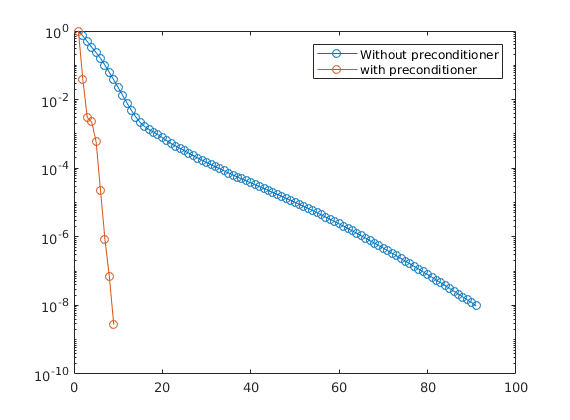
\includegraphics[scale=0.7]{../figs/PrecondDirichletLaplaceSeg.png}
%	\caption{Number of iteration in the resolution of the single layer integral equation with a mesh of size $N = 1600$.}
%	\label{FigureNitLaplaceDirichlet}
%\end{figure}
%
%\subsection{Hypersingular equation} 
%
%We now turn our attention to the equation 
%
%\begin{equation}
%N\mu = g
%\label{Nmu}
%\end{equation} 
%
%Similarly to the previous section and following again the idea of \cite{bruno2012second}, we consider a rescaled version of the hypersingular operator $N_\omega \isdef N \omega$ defined by
%
%\[N_\omega \mu = \lim_{\varepsilon\to 0}\int_{-1}^{1} n(y)\cdot\nabla G(x + \varepsilon n(x) - y) \sqrt{1-y^2} dy\]
%We can get the solution to equation \eqref{Nmu} by solving 
%\begin{equation}
%N_\omega \beta = u_N,
%\label{Nomegabeta}
%\end{equation}
%and letting $\mu = \omega \beta$. 
%We now show that $N_\omega$ can also be analyzed in our functional framework, using this time the spaces $U^s$. 
%\begin{Lem}
%	\label{lemIPP}
%	For any $\beta$, $\beta'$, one has 
%	\[\duality{N_\omega \beta}{ \beta'}_\omega = \duality{S_\omega \omega \partial_x \omega \beta}{\omega \partial_x \omega \beta'}_\frac{1}{\omega}.\]
%	\begin{proof}
%		It is sufficient to show this formula for $\beta$ and $\beta'$ in $U^{\infty}$ by density. Indeed, for such $\beta, \beta'$, both sides of the identity define continuous bilinear forms on $T^{\infty}$. We use the well-known integration by part formula
%		\[\duality{N u}{v} = \duality{S\partial_x u}{\partial_x v},\]
%		valid when $u$ and $v$ vanish at the extremities of the segment (see for example \cite{bruno2012second}). 
%		For a smooth $\beta$, we thus have
%		\[ \duality{N (\omega \beta)}{ (\omega \beta')} = \duality{S \partial_x(\omega \beta)}{\partial_x (\omega \beta')}\] 
%		which obviously implies the announced identity. 
%	\end{proof}
%\end{Lem}
%\begin{Prop}
%	$N_\omega$ is a positive definite, self-adjoint operator continuous from $U^s$ to $U^{s-1}$ for all real $s$. For all $n \in \N$, we have 
%	\[N_\omega U_n = \frac{n+1}{2}U_n.\]
%	Moreover, $-(\partial_x\omega)^2$ is also positive definite of order $2$.
%	\label{NUn}
%\end{Prop}
%\begin{proof}
%	From identity $T_{n+1}' = (n+1)U_n$ and Equation $\eqref{cheb1}$ we obtain
%	\begin{equation*}
%	\omega \partial_x \omega U_n = -(n+1) T_{n+1}.
%	\end{equation*}
%	Therefore, by \autoref{lemIPP}
%	\begin{eqnarray*}
%		\duality{N_\omega U_m}{U_n}_\omega & = & (n+1)(m+1)\duality{S_\omega T_{m+1}}{T_{n+1}}_\frac{1}{\omega}\\
%		&=& \delta_{m=n} \frac{n+1}{2}.	
%	\end{eqnarray*}
%	The fact that $-(\partial_x \omega)^2$ is self-adjoint positive definite of order $2$ is a consequence of Equation \eqref{cheb2}.
%\end{proof}
%	Like before, we have the following link between $U^{-1/2}$, $U^{1/2}$ and the usual Sobolev spaces. 
%
%As an application of this result, one can also derive the formal expansions as in \cite{jerez2012explicit}
%\[\frac{1}{(x-y)^2} = \sum_{n=0}^{+\infty} 2(n+1)U_n(x)U_n(y)\,,\]
%that lead, by applying for $(\partial_x\omega)^{-2}$ on both sides, to the following explicit kernel for the inverse of $N_\omega$:
%\[\ln\left(\dfrac{(y-x)^2 + (\omega(x) + \omega(y))^2}{2|x-y|}\right) = \sum_{n=0}^{+\infty} \dfrac{2 U_n(x) U_n(y)}{n+1}.\]
%Here instead, we give a simple expression of the inverse of $N_\omega$ as the inverse square root of a local operator:
%\begin{The} 
%	\label{the:NeumannInverseLaplace}
%	There holds 
%	\[N_\omega^2 = -\frac{1}{4}(\partial_x \omega)^2 \,.\]
%	The inverse of $N_\omega$ is therefore 
%	\begin{equation}
%	N_\omega^{-1} = 2\sqrt{-(\partial_x \omega)^{-2}}\,.
%	\end{equation}
%\end{The}
%In \autoref{TableNitTimeLaplaceNeumann}, we compare the number of iterations for the numerical resolution of Equation \eqref{Nomegabeta} by the method detailed in \autoref{sec:numerMeth} without preconditioner, and with a preconditioner given by $M^{-1} \left[B \right] M^{-1}$ where $M$ is the mass matrix and $\left[ B \right]$ is the Galerkin matrix of the operator $\sqrt{ -( \partial_x \omega)^{-2}}$. The right hand side in \eqref{Nomegabeta} is chosen as $u_N(x) = (x^2 + 0.001)^{1/2}, x \in (-1,1)$.
%
%\begin{table}[H]
%	\begin{center}
%		\begin{tabular}{|| m{4em} | m{4em} | m{4em} | m{4em} | m{4em}||} 
%			\hline
%			\multicolumn{1}{||c|}{ }&
%			\multicolumn{2}{c|}{with Prec.}&\multicolumn{2}{c||}{without Prec.}\\
%			\hline
%			$N$ & $n_{it}$& t(s) & $n_{it}$ & t(s)\\
%			\hline\hline
%			50 & 4 & 0.05 & 50 & 0.05\\
%			\hline
%			200 & 3 & 0.05 & 200 & 0.25\\
%			\hline
%			800 & 3 & 0.06 & 799 & 3.7 \\
%			\hline
%			3200 & 3 & 0.6 & 3007 & 630\\
%			\hline
%		\end{tabular}
%	\end{center}
%	\caption{Number of iteration and time needed for the numerical resolution of \eqref{Somegaalpha} using Galerkin finite elements with and without preconditioner.}
%	\label{TableNitTimeLaplaceNeumann}
%\end{table}
%\begin{figure}[H]
%	\centering
%	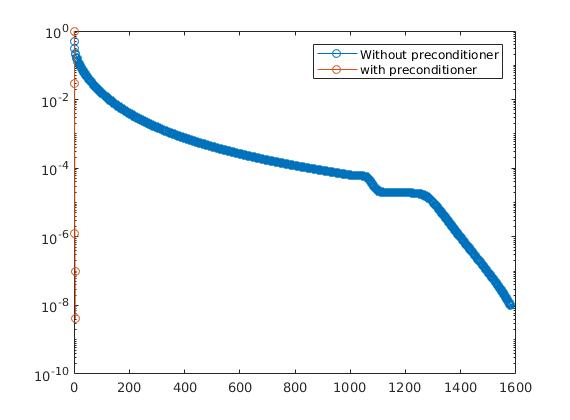
\includegraphics[scale=0.7]{../figs/PrecondNeumannLaplaceSeg.png}
%	\caption{Number of iteration in the resolution of the hypersingular  integral equation with a mesh of size $N = 1600$. The importance of preconditioning in this case is more obvious than in the case of the single-layer equation.}
%	\label{FigureNitLaplaceNeumann}
%\end{figure}
%
%\begin{Rem}
%	In \cite{bruno2012second}, the main theorem is equivalent to stating that $N_\omega S_\omega$ and $S_\omega N_\omega$ are bicontinuous operators in $T^s$, with a spectrum concentrated around $\frac{1}{4}$, which can be exploited for preconditioning purposes. It is shown that $N_\omega$ is continuous from $T^s$ to $T^{s-1}$ for all $s >1$ (in fact, this remains true for $s > \frac{1}{2}$). The two main arguments involved in the proof are the explicit expression of $N_\omega T_n$ and the continuity of the adjoint of the Cesaro operator in $l^2(\N)$. The same arguments can be used to prove that $S_\omega$ is also a bicontinuous operator from $U^s$ to $U^{s+1}$ for all $s > 1/2$. 
%\end{Rem}



%\section{Helmholtz equation}

%	In this section, we introduce preconditioners for the integral equations on $\Gamma = (-1,1)$ for the Helmholtz equation. Recall the definition of the single layer and hypersingular operators, $S_k$ and $N_k$, given in \eqref{defSk} and \eqref{defNk}, and the integral equations for the Dirichlet and Neumann problems, \eqref{Sklambda} and \eqref{Nkmu}. As before, let $S_{k,\omega} \isdef S_k \frac{1}{\omega}$ and $N_{k,\omega} \isdef N_k \omega$. We begin by establishing the following result:
%	
%	\begin{The}
%		\label{Commutations}
%		The following commutations hold:
%		\[S_{k,\omega} \left[-(\omega \partial_x)^2 - k^2\omega^2\right] =  \left[-(\omega \partial_x)^2 - k^2\omega^2\right]S_{k,\omega},\]
%		\[N_{k,\omega} \left[-(\partial_x \omega)^2 - k^2\omega^2\right] =  \left[-(\partial_x \omega)^2 - k^2\omega^2\right]N_{k,\omega}.\]
%		\begin{proof}
%			We start with the first commutation. Since $(\omega \partial_x)^2$ is self adjoint and symmetric, we have 
%			\[S_{k,\omega} (\omega \partial_x)^2 = \int_{-1}^{1} \frac{(\omega_y \partial_y)^2 \left[G_k(x-y)\right] u(y)}{\omega(y)},\]
%			where we use the notation $\omega_y$ and $\partial_y$ to emphasize the dependence in the variable $y$. 
%			Thus, 
%			\[S_{k,\omega} (\omega \partial_x)^2 - (\omega \partial_x)^2 S_{k,\omega} = \int_{-1}^{1} \frac{D_k(x,y)u(y)}{\omega(y)},\]
%			where $D_k(x,y) \isdef \left[(\omega_y \partial_y)^2 - (\omega_x \partial_x)^2\right] \left[G_k(x-y)\right]$. 
%			One has 
%			\[D_k(x,y) = G_k''(x-y) (\omega^2_y - \omega^2_x) + G_k'(x-y)(y + x).\]
%			Since $G_k$ is a solution of the Helmholtz equation, we have for all $(x \neq y) \in \R^2$ 
%			\[G_k'(x-y) = (y-x)(G_k''(x-y) + k^2G(x-y)),\]
%			thus
%			\[D_k(x,y) = G_k''(x-y)\left(\omega^2_y - \omega_x^2 + y^2 - x^2\right) + k^2(y^2 - x^2)G_k(x-y) . \]
%			A careful analysis shows that no Dirac mass appears in the previous formula, that is, the previous formula is an equality of two functions in $T^{-\infty}$. 
%			Note that $y^2 - x^2 = \omega_x^2 - \omega_y^2$ so the first term vanishes and we find
%			\[S_{k,\omega} (\omega \partial_x)^2 - (\omega \partial_x)^2 S_{k,\omega} =  k^2\left(\omega^2 S_{k,\omega} -S_{k,\omega} \omega^2 \right). \]
%			The proof of the second commutation is postponed to \autoref{ann:commut}. 
%		\end{proof}
%	\end{The}
%	
%	This theorem implies that the operators $S_{k,\omega}$ and $N_{k,\omega}$ share the same eigenvectors as, respectively, $\left[-(\omega \partial_x)^2 - k^2\omega^2\right]$ and $ \left[-(\partial_x \omega)^2 - k^2\omega^2\right]$. We can look for eigenfunctions of the operator $\left[ -(\omega \partial_x)^2 - k^2\omega^2\right]$, to find a diagonal basis for $S_{k,\omega}$. They are the solutions to the differential equation 
%	\[ (1-x^2) y'' - x y' - k^2 \omega^2 y = \lambda y.\]
%	Once we set $x = \cos \theta$, $\tilde{y}(\theta) = y(x)$,  $q = \frac{k^2}{4}$, $a = \lambda + 2q$, $\tilde{y}$ is a solution of the standard Mathieu equation 
%	\begin{equation}
%	\label{MatthieuEq}
%		\tilde{y}'' + (a - 2q \cos(2\theta)) \tilde{y} = 0.
%	\end{equation}
%	There are a discrete set of values $a_{2n}(q)$ for which this equation possesses an even and $2\pi$ periodic function. The corresponding solution is known as the Mathieu cosine, and usually denoted by $\textup{ce}_n$. Here, we use the notation $\textup{ce}^k_n$ to emphasize the dependency in the parameter $k = \sqrt{2q}$ of those functions. The normalization is taken as
%	\[ \int_{0}^{2\pi} \textup{ce}^k_n(\theta)^2 d\theta = \pi.\]
% 	They satisfy
%	\[ \int_{-\pi}^{\pi}\textup{ce}^k_n(\theta) \textup{ce}^k_m(\theta) = \pi \delta_{m,n}.\]
%	Any even $2\pi$ periodic function in $L^2(-\pi,\pi)$ can be expanded along the functions $\textup{ce}_n$, with the coefficients obtained by orthonormal projection. Letting 
%	\[T_{n}^k \isdef \textup{ce}^k_n(\arccos(x)),\]
%	in analogy to the zero-frequency case, we have
%	\[\left[-(\omega \partial_x)^2 - k^2\omega^2\right] T_{n}^k = \lambda_{n,k}^2 T_{n}^k.\]
%	For large $n$, using the general results from the theory of Hill's equations (see \cite[eq. 28.29.21]{NIST:DLMF}) we have the following asymptotic formula for $\lambda_{n,k}$:
%	\[ \lambda_{n,k}^2 = n^2 - \frac{k^4}{16n^2} +o \left(n^{-2}\right). \]
%	The first commutation established in \autoref{Commutations} implies that the Matthieu cosines are also the eigenfunctions of the single-layer operator. An equivalent statement is given in \cite[Thm 4.2]{betcke2014spectral}, if we allow the degenerate case $\mu = 0$. 
%	A similar analysis can be applied to the hypersingular operator. The eigenfunctions of $\left[(\partial_x \omega)^2 - k^2 \omega^2\right]$ are given by 
%	\[U_n^k \isdef \frac{\textup{se}_n^k(\arccos(x))}{\omega(x)}\]
%	where $\textup{se}_n^k$ are the so-called Matthieu sines, which also satisfy the Matthieu differential equation \eqref{MatthieuEq}, but with the condition that they must be odd $2\pi$ periodic functions. 
%	Unfortunately, the lack of knowledge about the eigenvalues of $S_{k,\omega}$ and $N_{k,\omega}$ prevents us from applying a similar analysis as that performed in the first part of this work. Instead, we will perform a perturbation analysis, much like \cite{bruno2012second}.
